\documentclass[10pt,twocolumn]{article}

% use the oxycomps style file
\usepackage{oxycomps}

% usage: \fixme[comments describing issue]{text to be fixed}
% define \fixme as not doing anything special
\newcommand{\fixme}[2][]{#2}
% overwrite it so it shows up as red
\renewcommand{\fixme}[2][]{\textcolor{red}{#2}}
% overwrite it again so related text shows as footnotes
%\renewcommand{\fixme}[2][]{\textcolor{red}{#2\footnote{#1}}}

% read references.bib for the bibtex data
\bibliography{references}

% include metadata in the generated pdf file
\pdfinfo{
    /Title (Git and LaTeX Worksheet)
    /Author (Justin Li)
}

% set the title and author information
\title{Git and \LaTeX Worksheet}
\author{Justin Li}
\affiliation{Occidental College}
\email{justinnhli@oxy.edu}

\begin{document}

\maketitle

\section{Instructions}

This worksheet is due March 1, 2025 at midnight, to be submitted as a GitHub repository URL to Canvas. The repository should contain all files requires to compile this worksheet with your answers. You should only change this \texttt{document.tex} file and the  \texttt{references.bib} file; do not change any other file in this starting repository. You should not use any additional packages, and are not allowed to use the \texttt{{\textbackslash}usepackage\{\}} command. Additionally, the output should be formatted correctly: your answers should be appropriately nested under the questions, command-line commands should be in monospace, and images should be positioned appropriately.

Gary.w
\section{Git Questions}

\subsection{General questions}

\begin{enumerate}
    \item What is a version control system? Why are they useful?

    \medskip
    Version control systems help manage changes to files and code by tracking changes and maintaining a history of all edits. Allows you to back up old versions of files and allow for parallel development without incurring risks. 
    \medskip
    
    \item What is the difference between git and GitHub?

    \medskip
    git is a version control system  while github is a cloud based platform that hosts git repositories. Provides a centralized location to store git repositories online.
    \medskip
    
    \item What is a repository?

    \medskip
    a digital storage location fora project containing its files, code and version history it can be locally hosted or hosted remotely on platforms like github. A repository stores changes and tracks the edit history.
    \medskip
    
    \item What is a commit?

    \medskip
    A commit is a snapshot/version of your project you save. When committing git saves the changes made since the last commit and is assigned a unique hash to id and tag that version of the project. The commit is then linked to the previous one creating a chain of history.
    \medskip
    
    \item What is the commit graph?

    \medskip
    A commit graph is a representation of the commit history of a repository it shows how commits are connected including branches merges and the sequence of commits. The graph is directed and acyclic where nodes represent commits and nodes have one parent if its a normal commit or multiple parents if the commit is a merge
    \medskip
    
    \item What is your preferred local git client (eg., command line, GitHub Desktop, GitKraken, etc.)?

    \medskip
    Github desktop
    \medskip
    
\end{enumerate}

\subsection{Local Usage}

\begin{enumerate}
\item What is the difference between adding a file to the staging area and committing a file?

\medskip
adding a file to the staging area prepares it for the next commit, it only affects selected files whereas a commit affects everything. adding a file to the staging area is not permanent and can be easily modifed, a commit on the other hand is usually permanent.
\medskip

\item What is a commit message, and why is it important for them to be meaningful?

\medskip
a commit message is  a short description attached to a commit explaining the purpose of the commit. It can be helpful to give context and clarity to commits helping with debugging and collaborations as what the commit has done can be easily conveyed.
\medskip

\item Starting with an empty repository, what sequence of commands/actions would result in the following commit graph? You may give a sequence of \texttt{git} commands, or describe (with screenshots) how you would do this in your preferred graphical git interface.
\begin{verbatim}
A---B---C---D
\end{verbatim}

\medskip
open github desktop and click file then new repository and enter a repo name and the github folder is chosen as default but can be changed. Create the repository and create a new file in that folder. Go to the github desktop and add a commit message then click commit to main. Modify the file then commit a gain the same way. Do this in total 4 times to create the commit graph

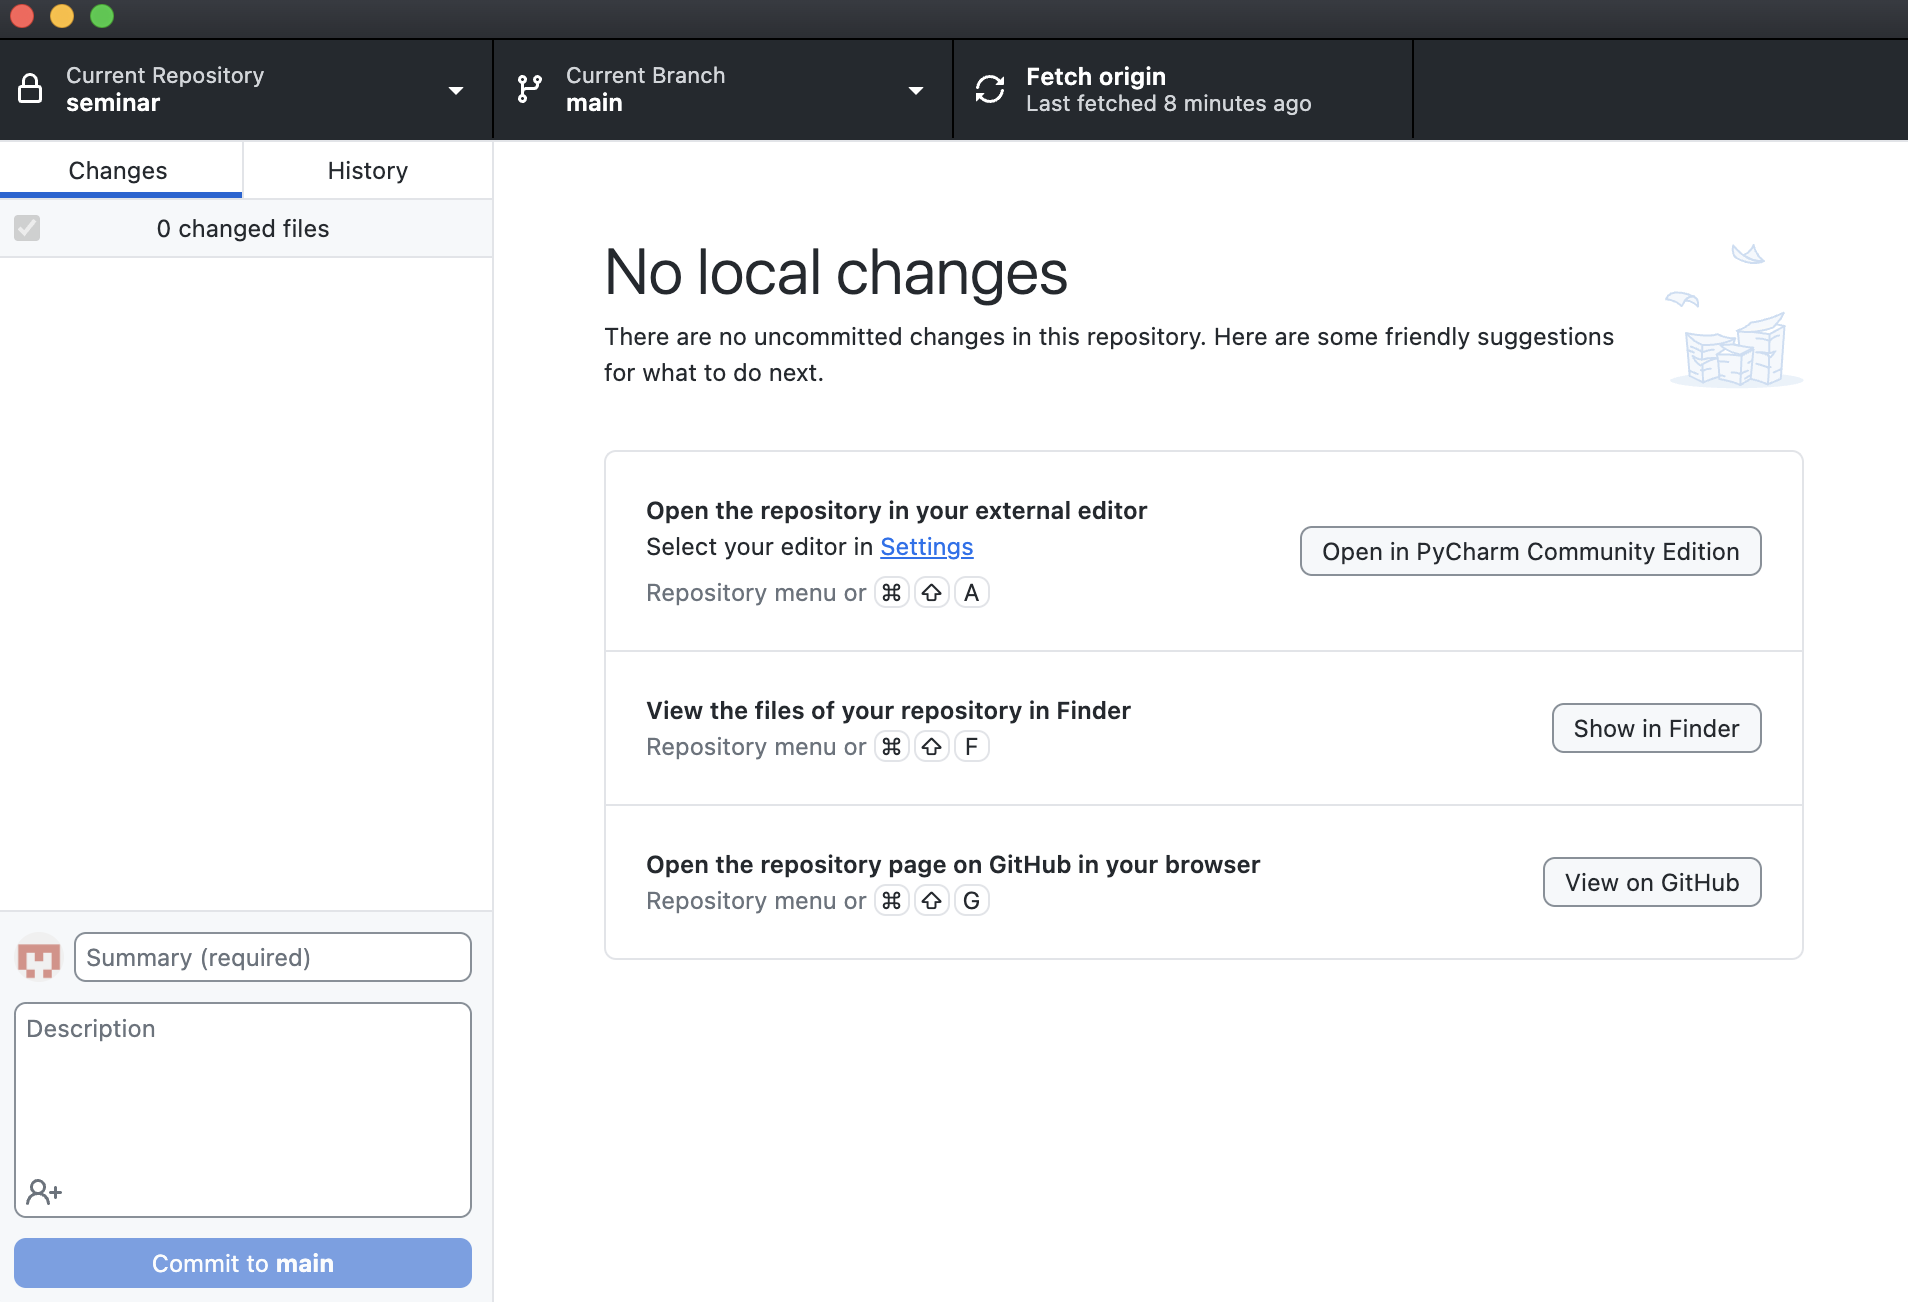
\includegraphics[width=\linewidth]{1.png}
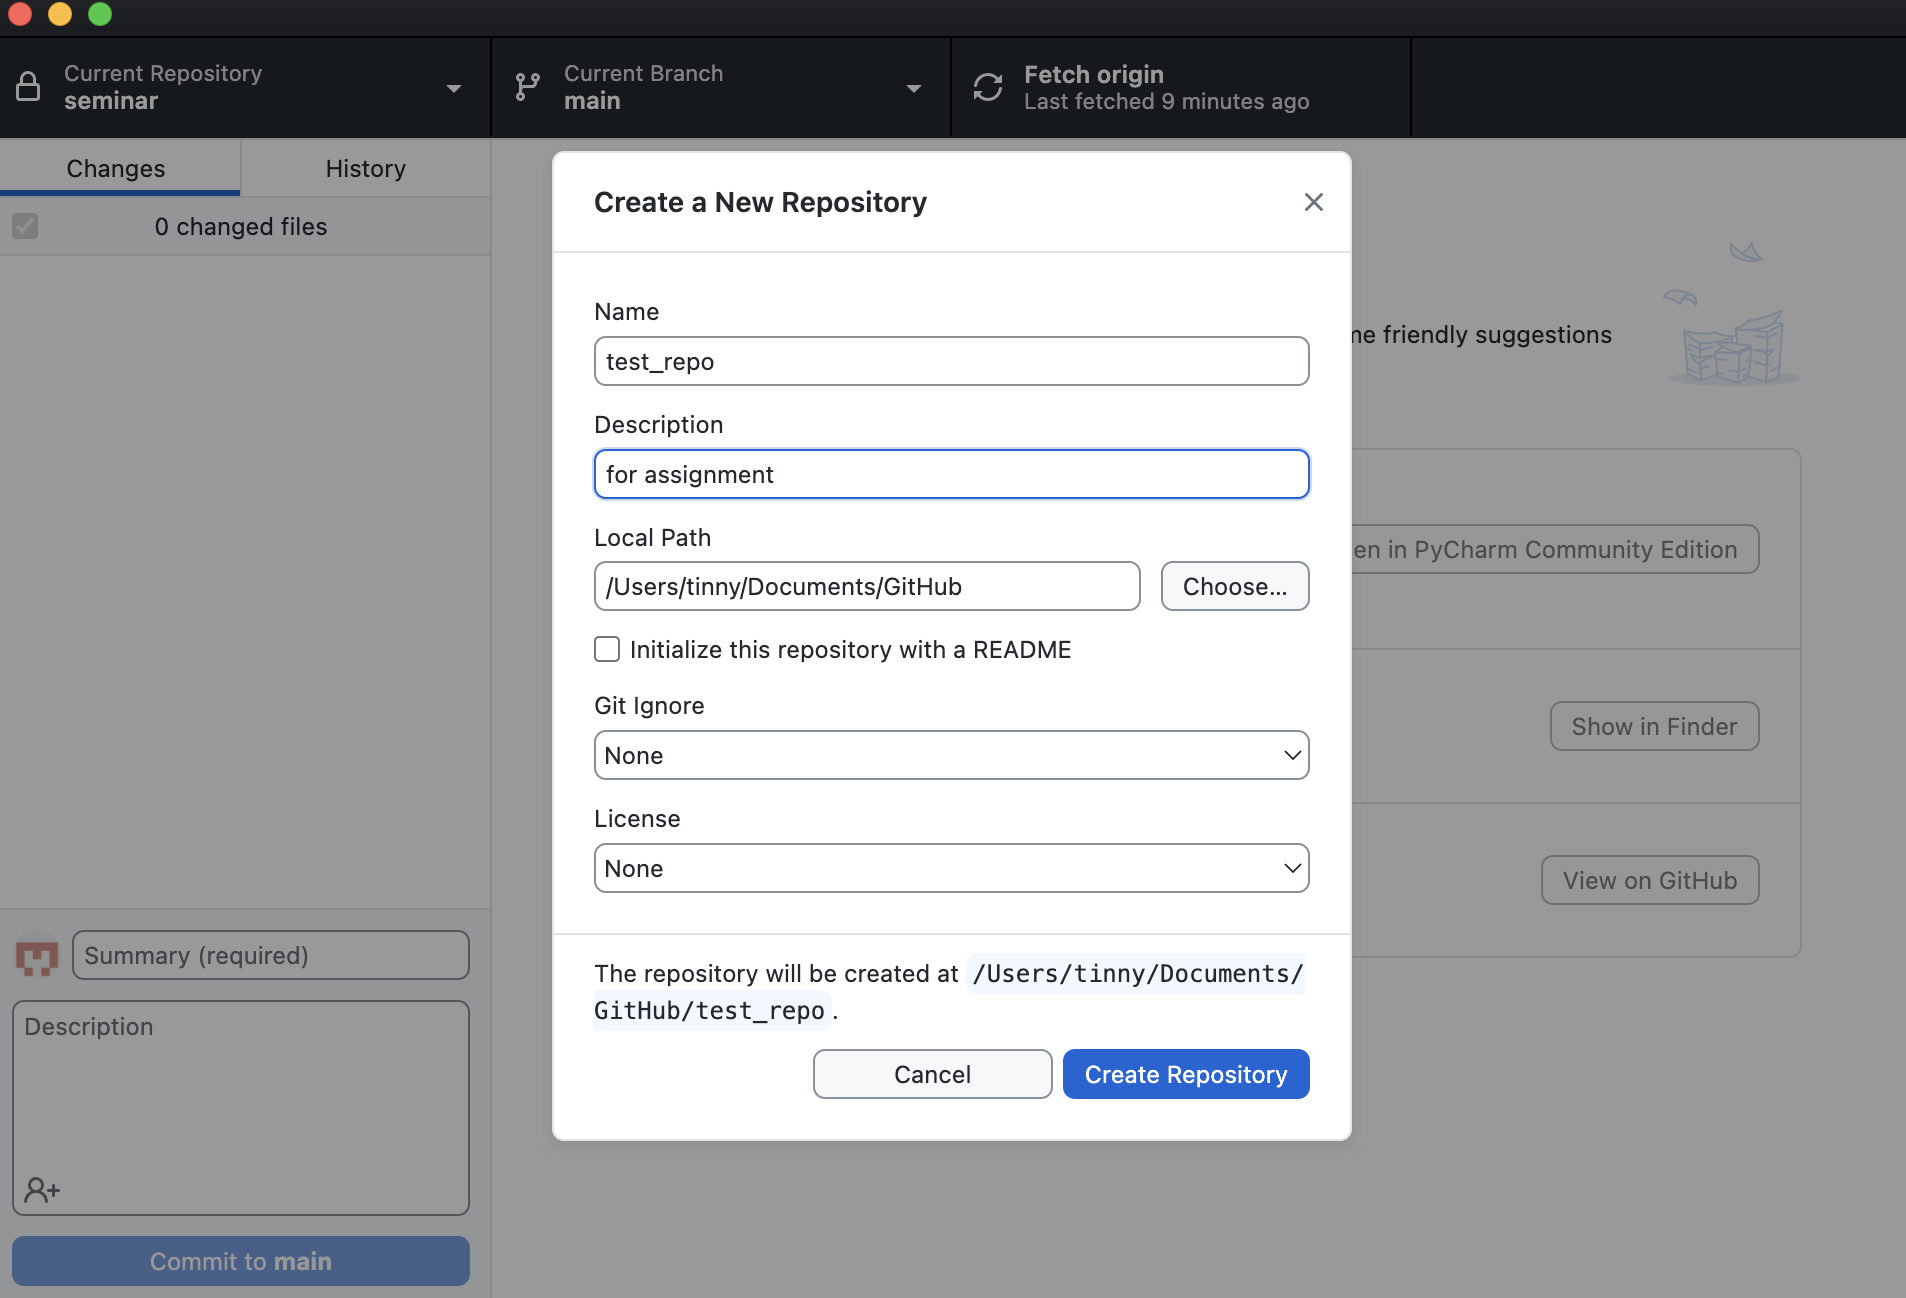
\includegraphics[width=\linewidth]{2.png}
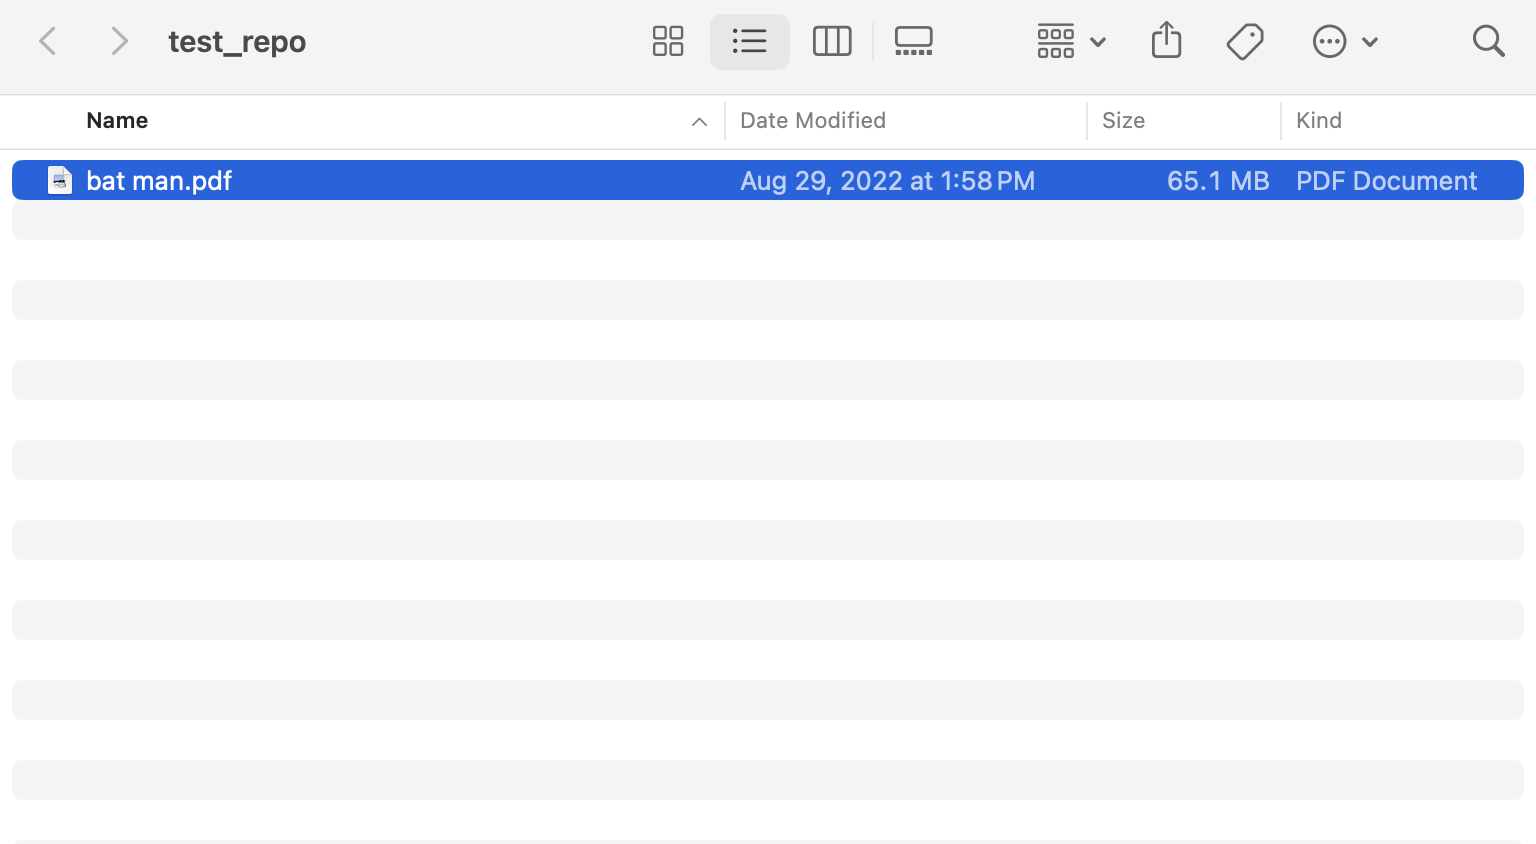
\includegraphics[width=\linewidth]{3.png}
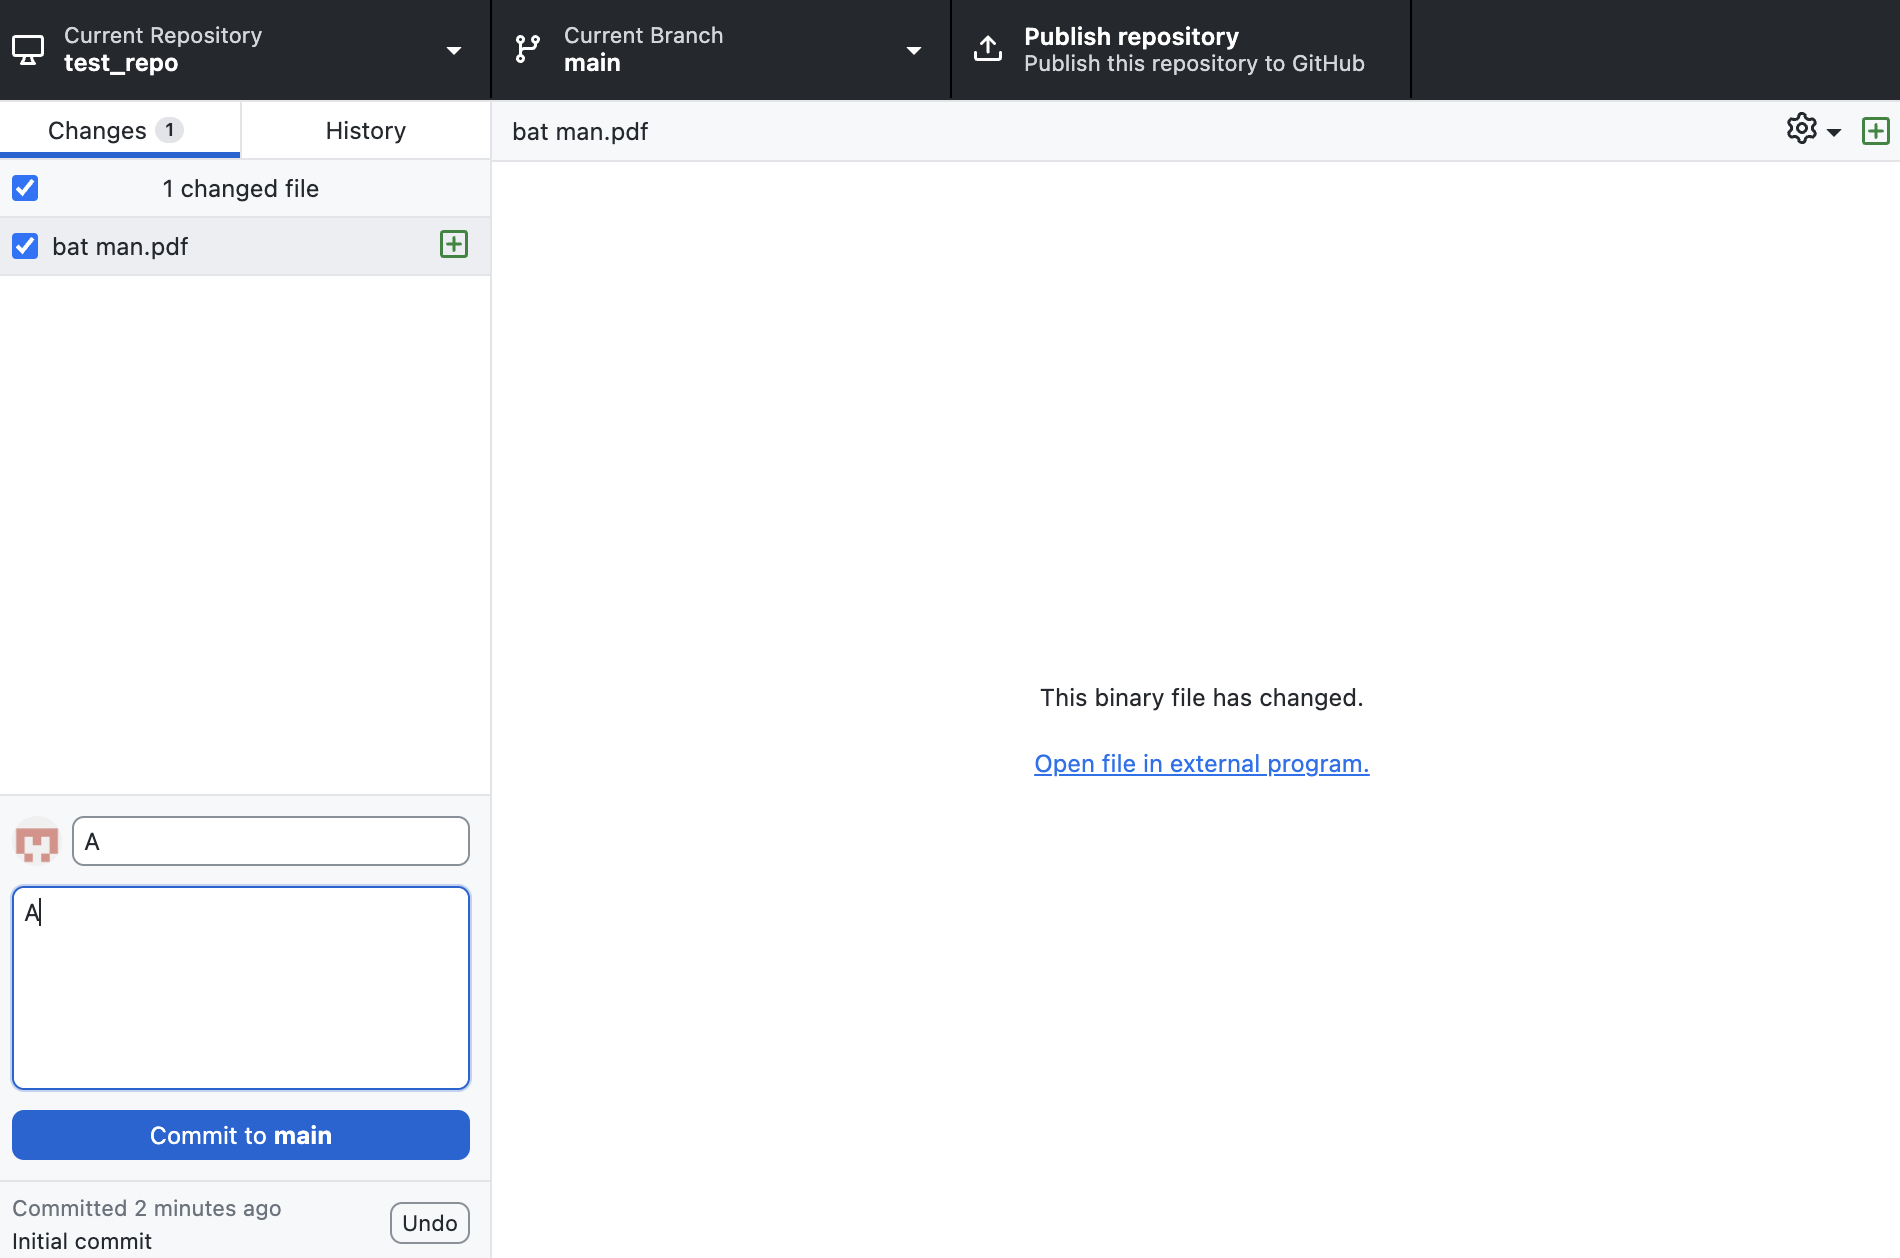
\includegraphics[width=\linewidth]{4.png}

\medskip

\item If you are currently at commit D above, how would you recover code from commit B? What sequence of commands/actions would let you do so? You may give a sequence of \texttt{git} command-line commands, or describe (with screenshots) how you would do this in your preferred graphical git interface. Assume the commit hashes are AAAAAA..., BBBBBB..., etc.

\medskip

open github desktop and click the history tab, find commit b and right click it , then click branch from this commit to create a branch so you can work on B while preserving the previous commits.

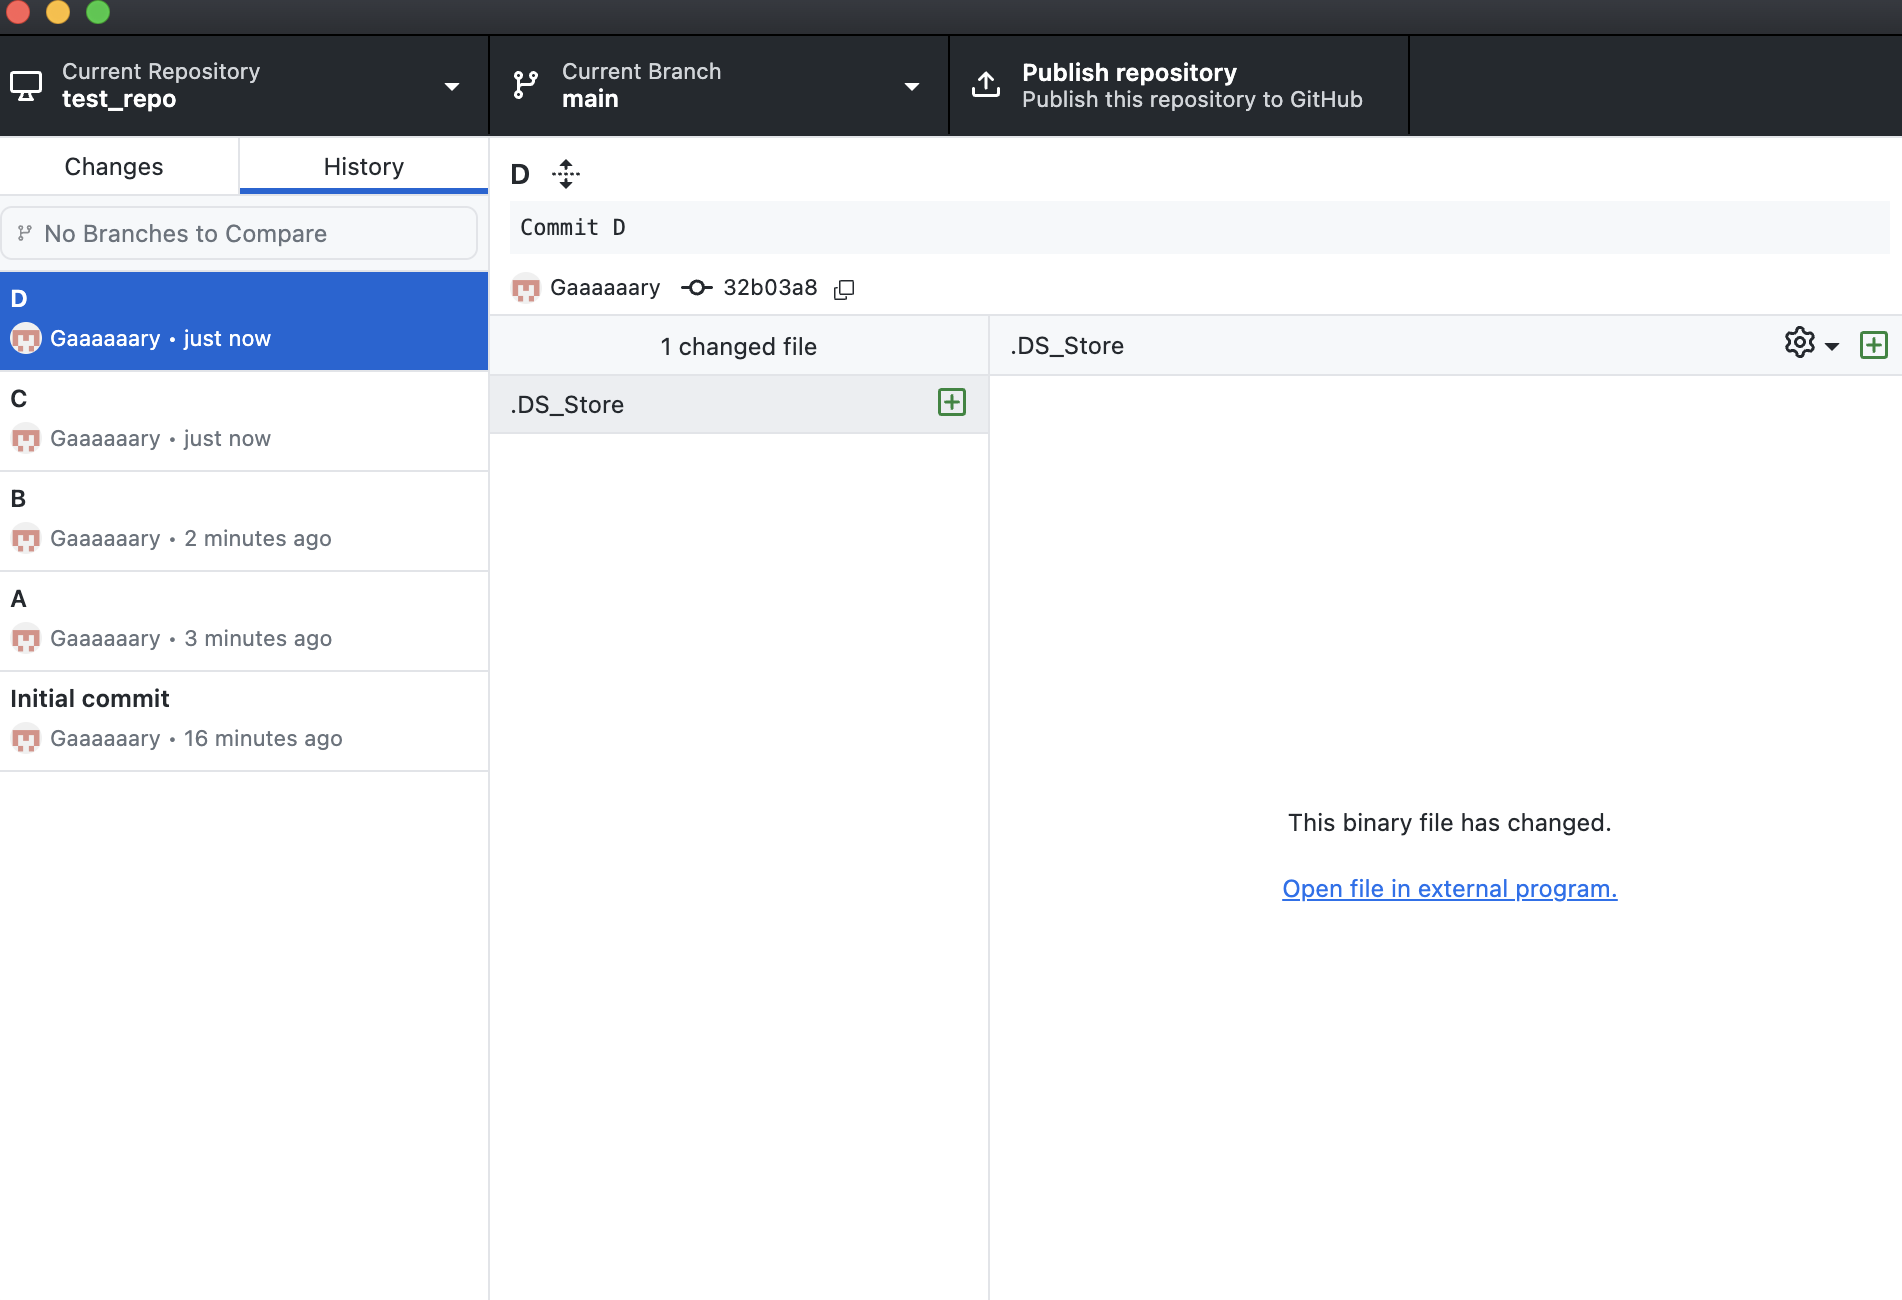
\includegraphics[width=\linewidth]{5.png}
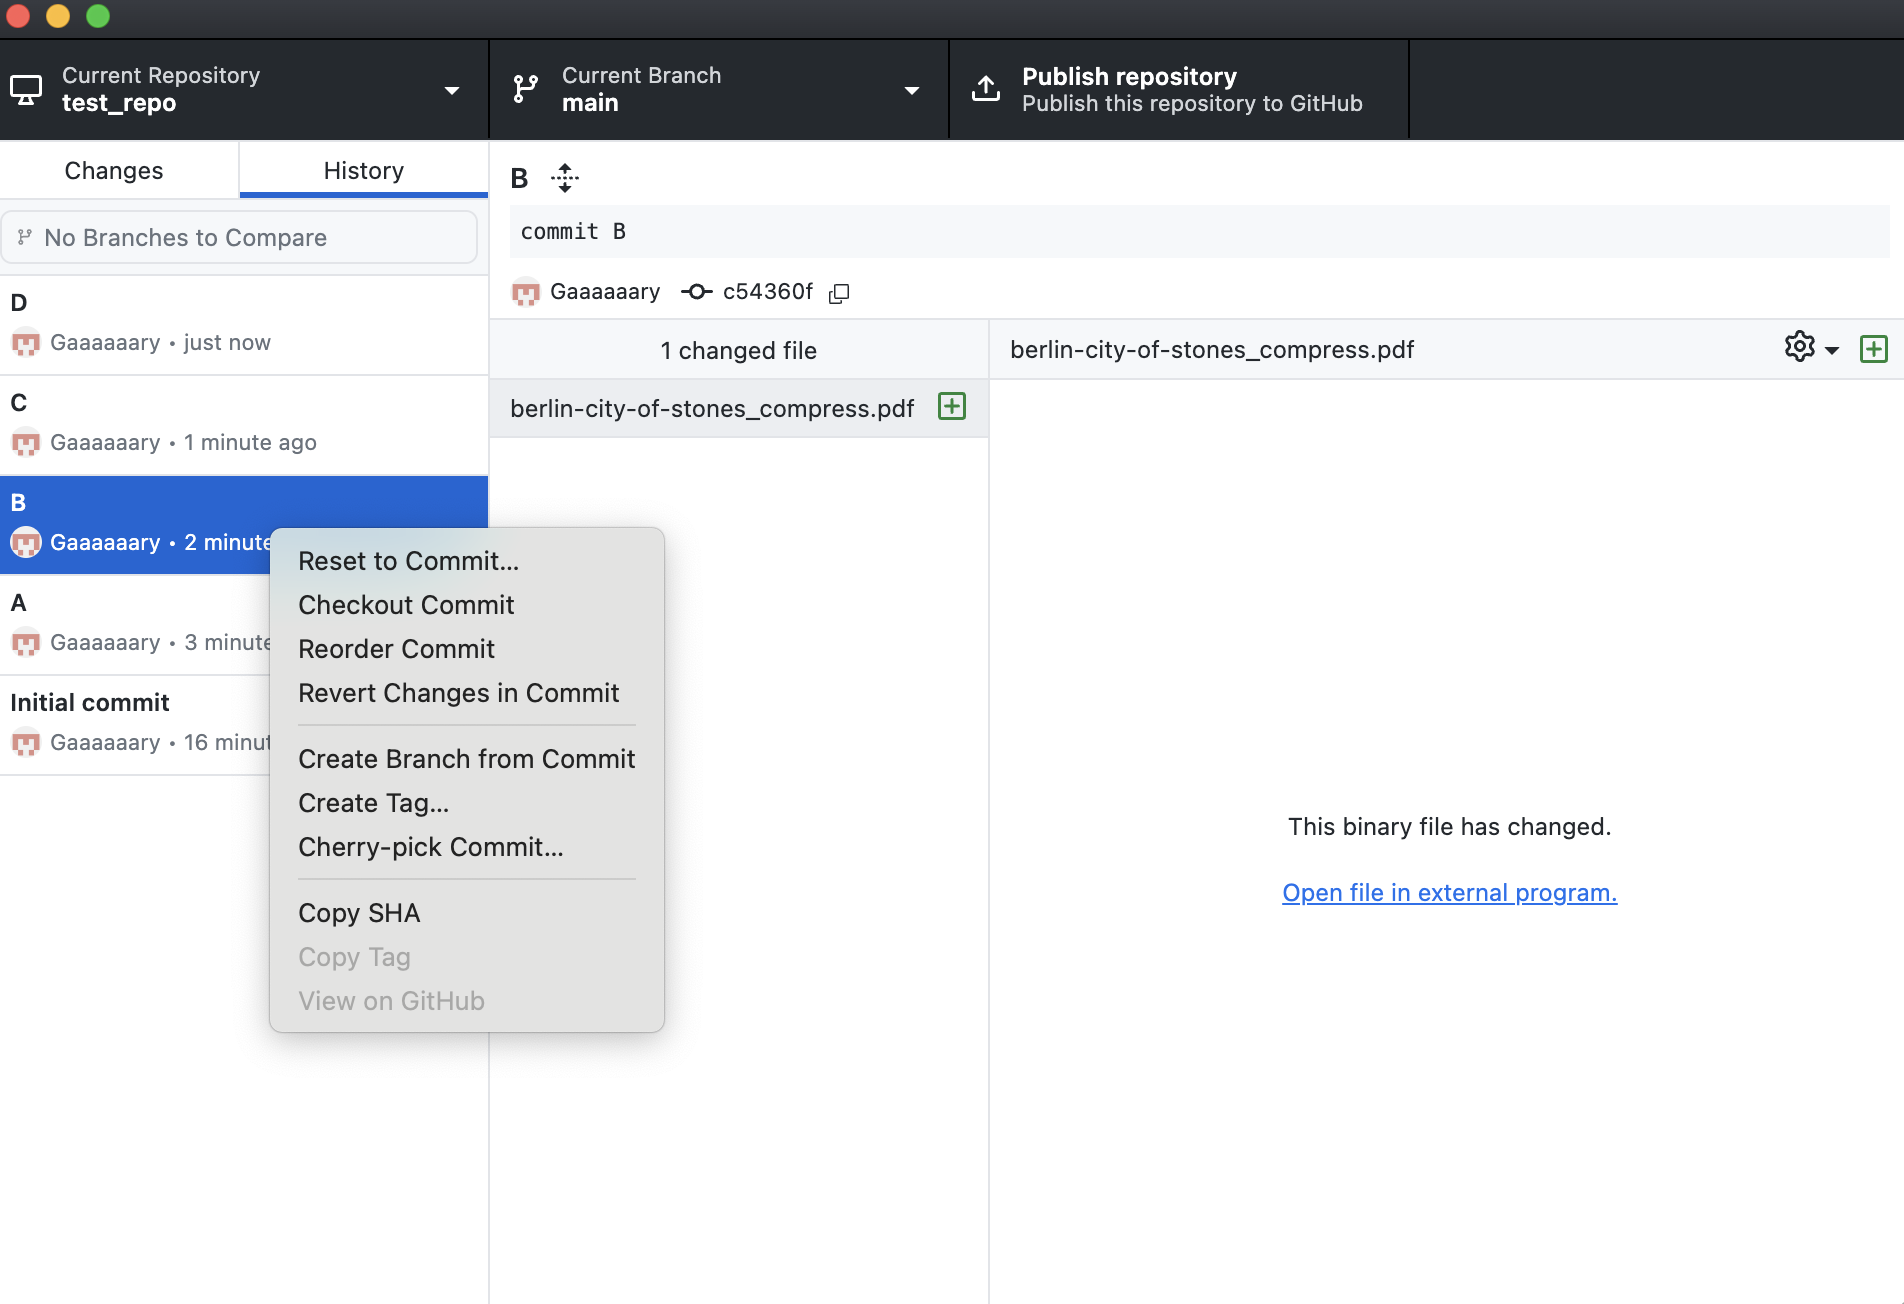
\includegraphics[width=\linewidth]{6.png}
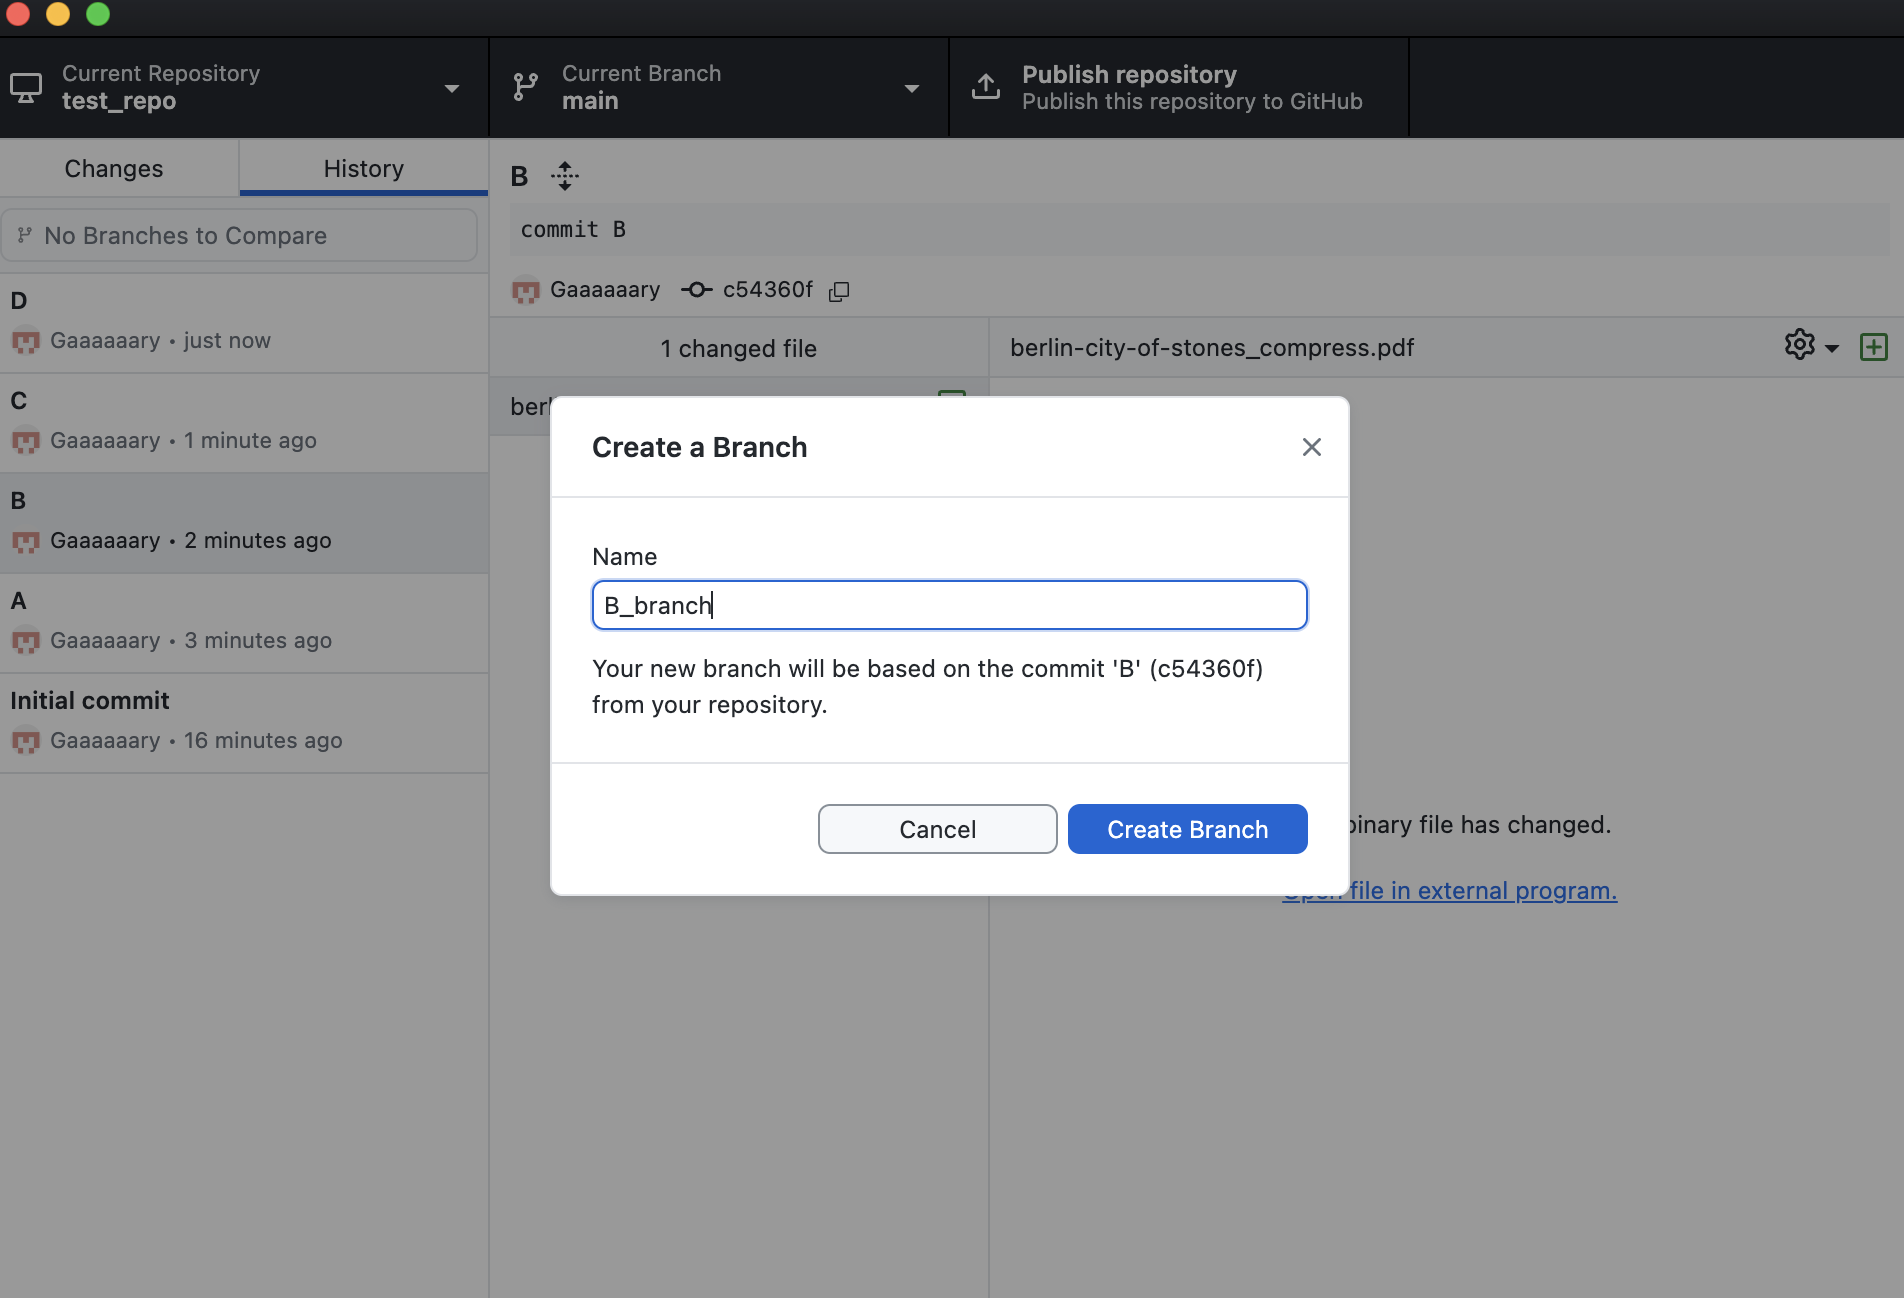
\includegraphics[width=\linewidth]{7.png}


\medskip

\item Imagine you created a git repository for your project, but only commit your changes once a week on Sundays. You got your code working on Tuesday, but then broke your code on Friday. What can you do to get the working version of your code back?
\end{enumerate}

\medskip
you can either discard all changes after Sunday by resetting the repository to last Sunday commit, or you can stash the current state of the repository, restore the repository to the Sunday commit. If you stashed the working code on Tuesday, you can also restore that.


\medskip

\subsection{Branching and Merging}

\begin{enumerate}
\item What is a branch? Why are they useful?

\medskip
A branch is a separate line of development that allows people to work with older version of the project without interfering with the main version of the project. Branches can be formed from any previous commit. They are useful for parallel development, experimenting and easier collaboration as people can each work on there own isolated code then merge back together.
\medskip

\item Starting with an empty repository, what sequence of commands/actions would result in the following commit graph? You may give a sequence of \texttt{git} command-line commands, or describe (with screenshots) how you would do this in your preferred graphical git interface.
\begin{verbatim}
A---B---C---D
     \
      E---F
\end{verbatim}

\medskip
question 3 in 2.2 shows the steps to achieving the A, B, C, D commit graph, from there create a branch as shown in 2.2 question 4. From there you will be automatically be put in branch in, the make the changes and commit again making sure the tab says branch E.

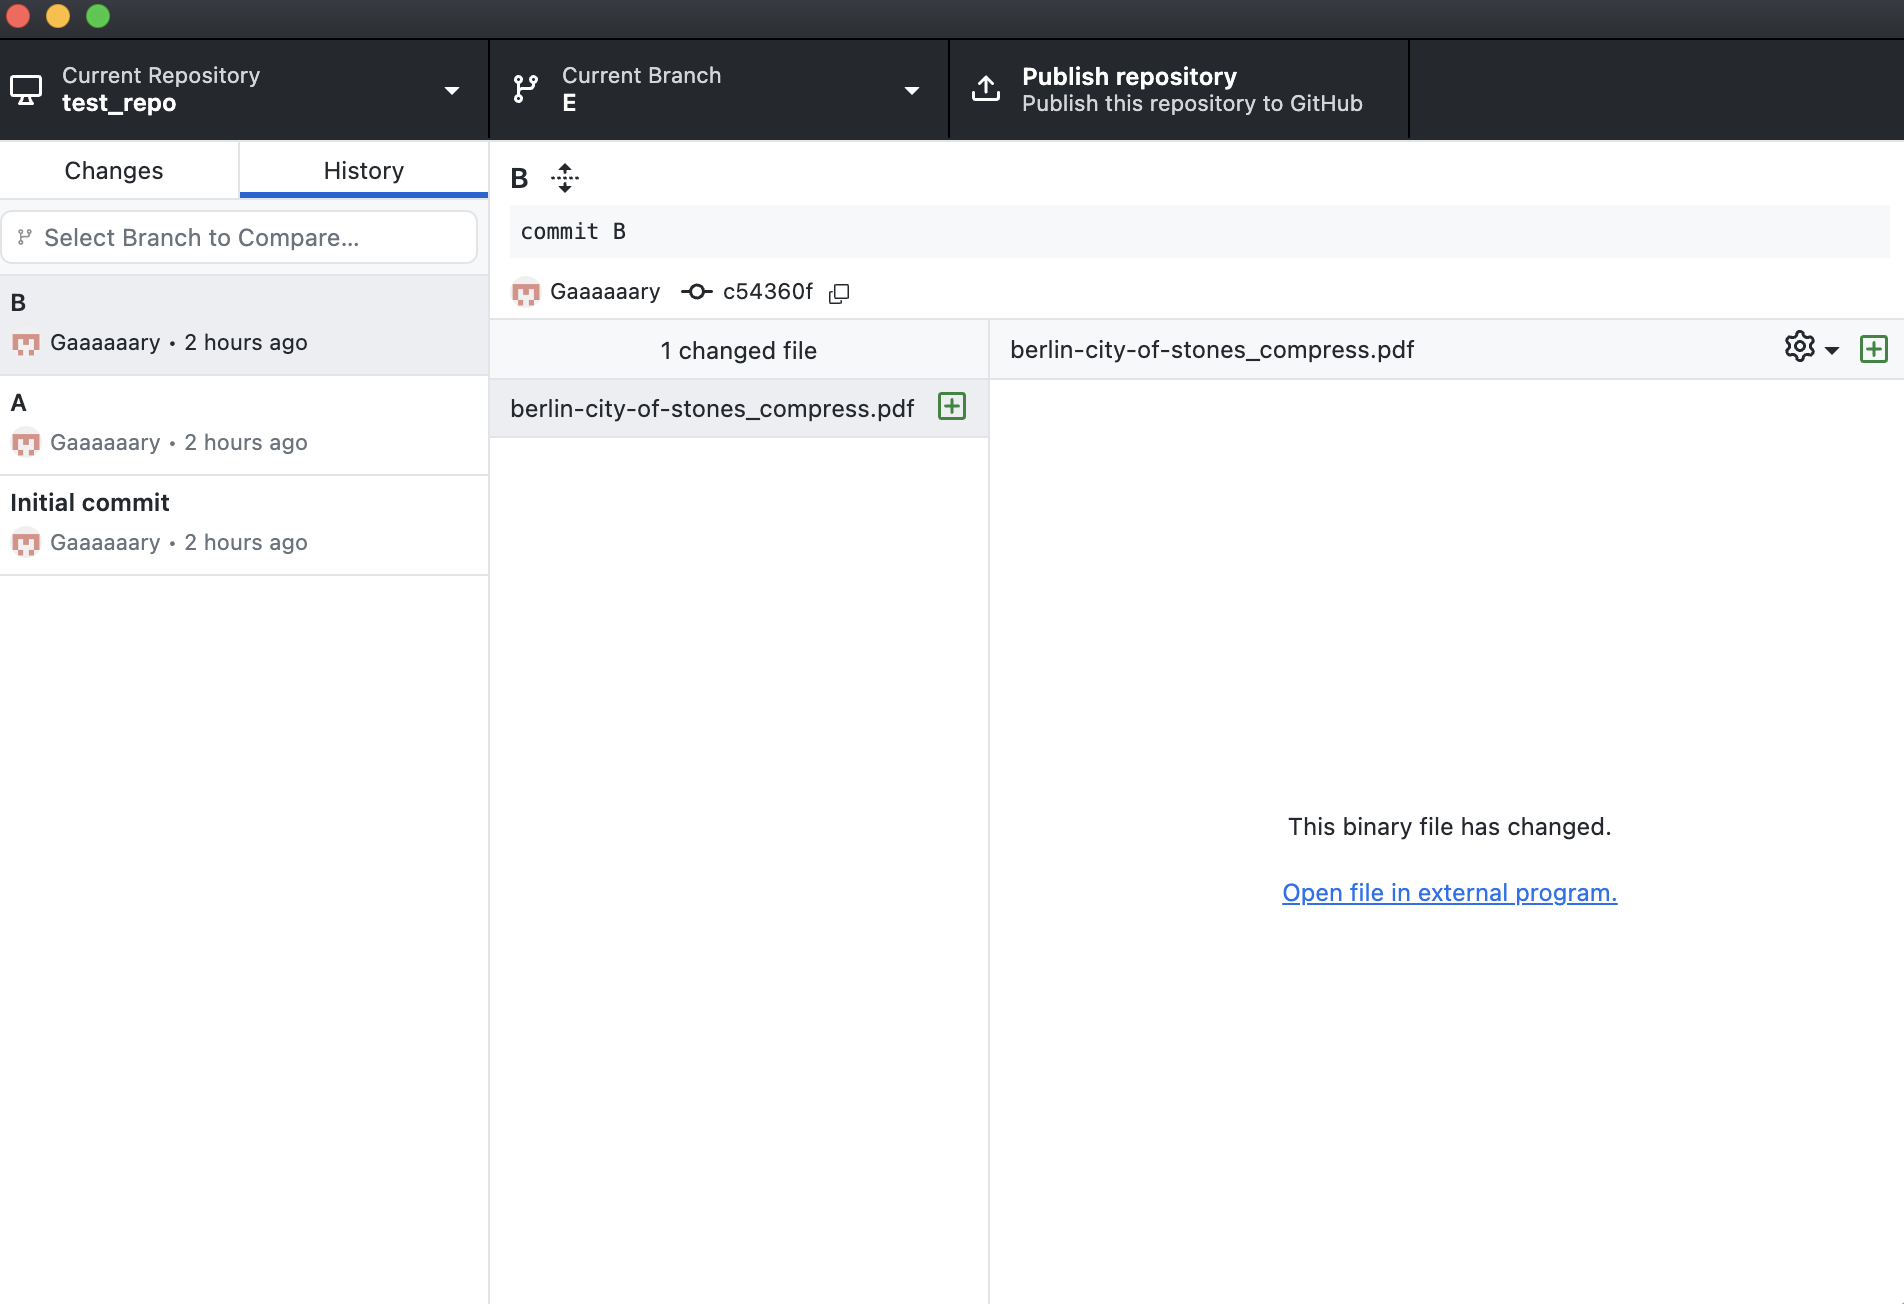
\includegraphics[width=\linewidth]{8.png}
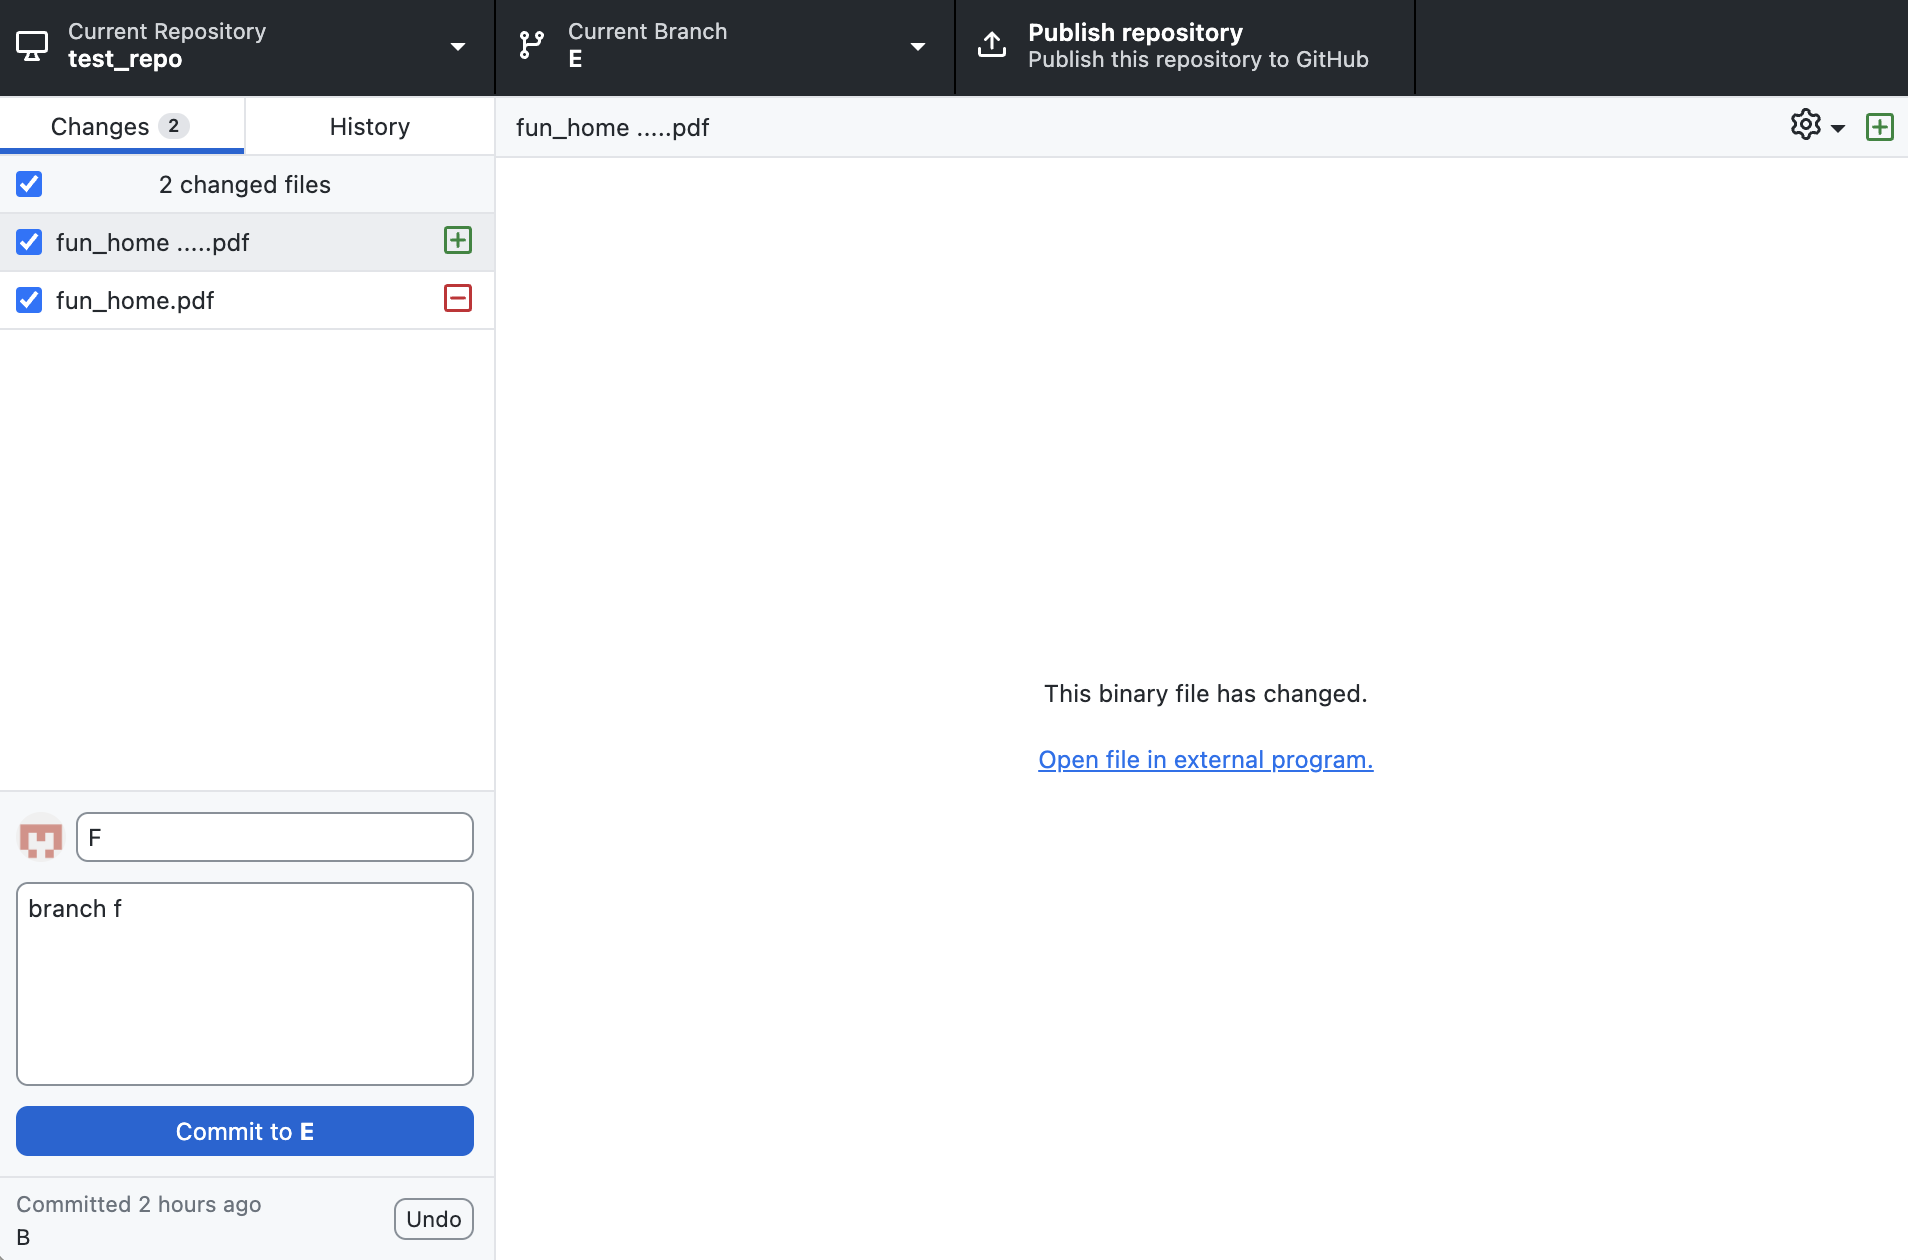
\includegraphics[width=\linewidth]{9.png}
\medskip

\item Why is a merge? Why are they useful?

\medskip
A merge is the process of combining the changes from branches. It integrates the work done from different branches but if there conflicts in the code they will need to be resolved manually. Merging is usually done when an isolated feature is fully developed and ready to be integrated into the main code. Merging is useful for collaboration as developers can independently work on their own sections then merge the code to combine it.
\medskip

\item Imagine you are currently at commit D above. What sequence of commands/actions would result in the following commit graph? You may give a sequence of \texttt{git} commands, or describe (with screenshots) how you would do this in your preferred graphical git interface.
\begin{verbatim}
A---B---C---D---G
     \         /
      E---F---/
\end{verbatim}

\medskip
from question 4 of 2.3 obtain the commit graph, now switch to the main branch by clicking the branch tab, then click the merge into branch and select E then merge the branches
\medskip

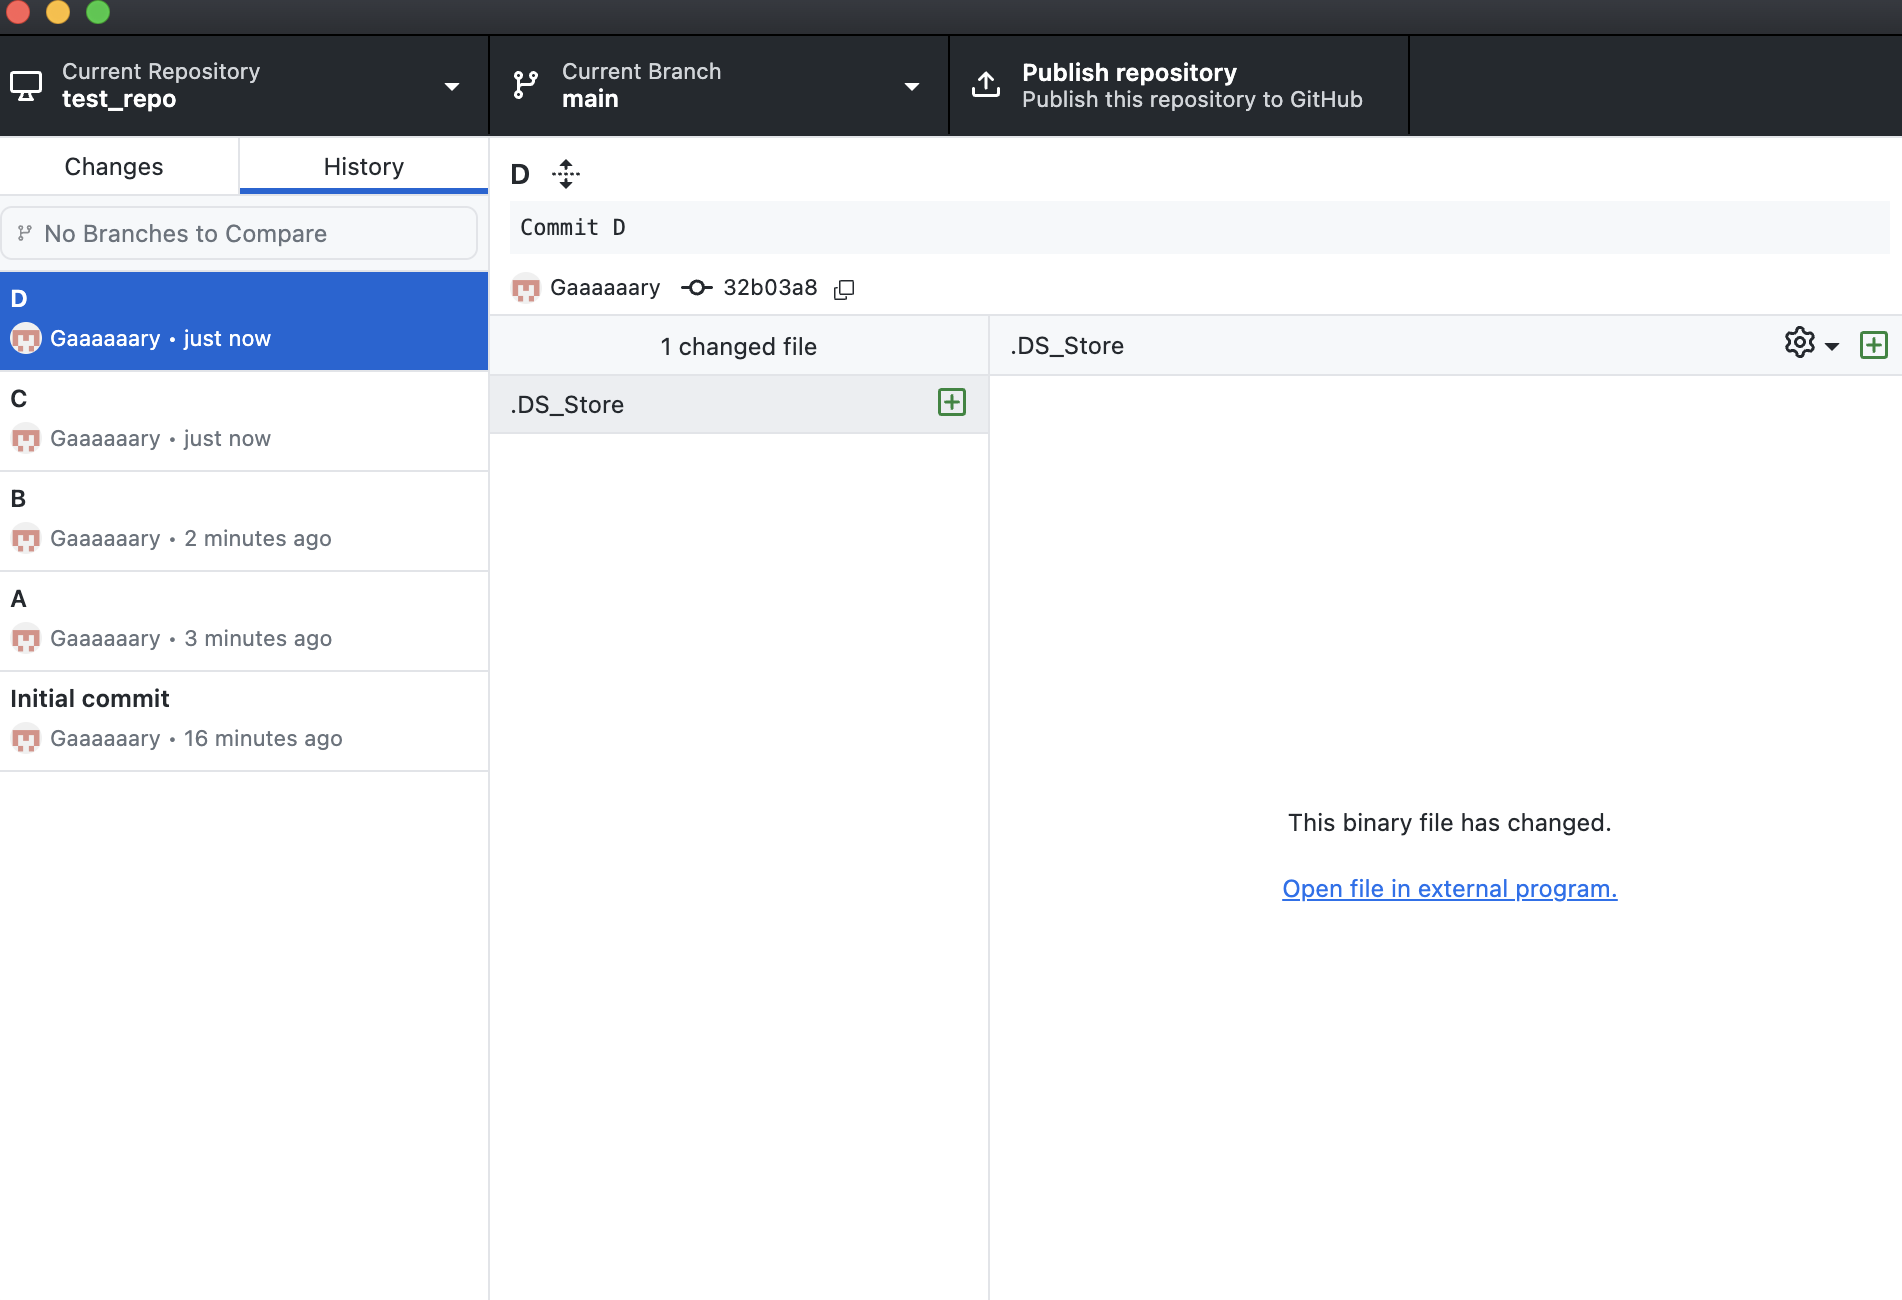
\includegraphics[width=\linewidth]{10.png}
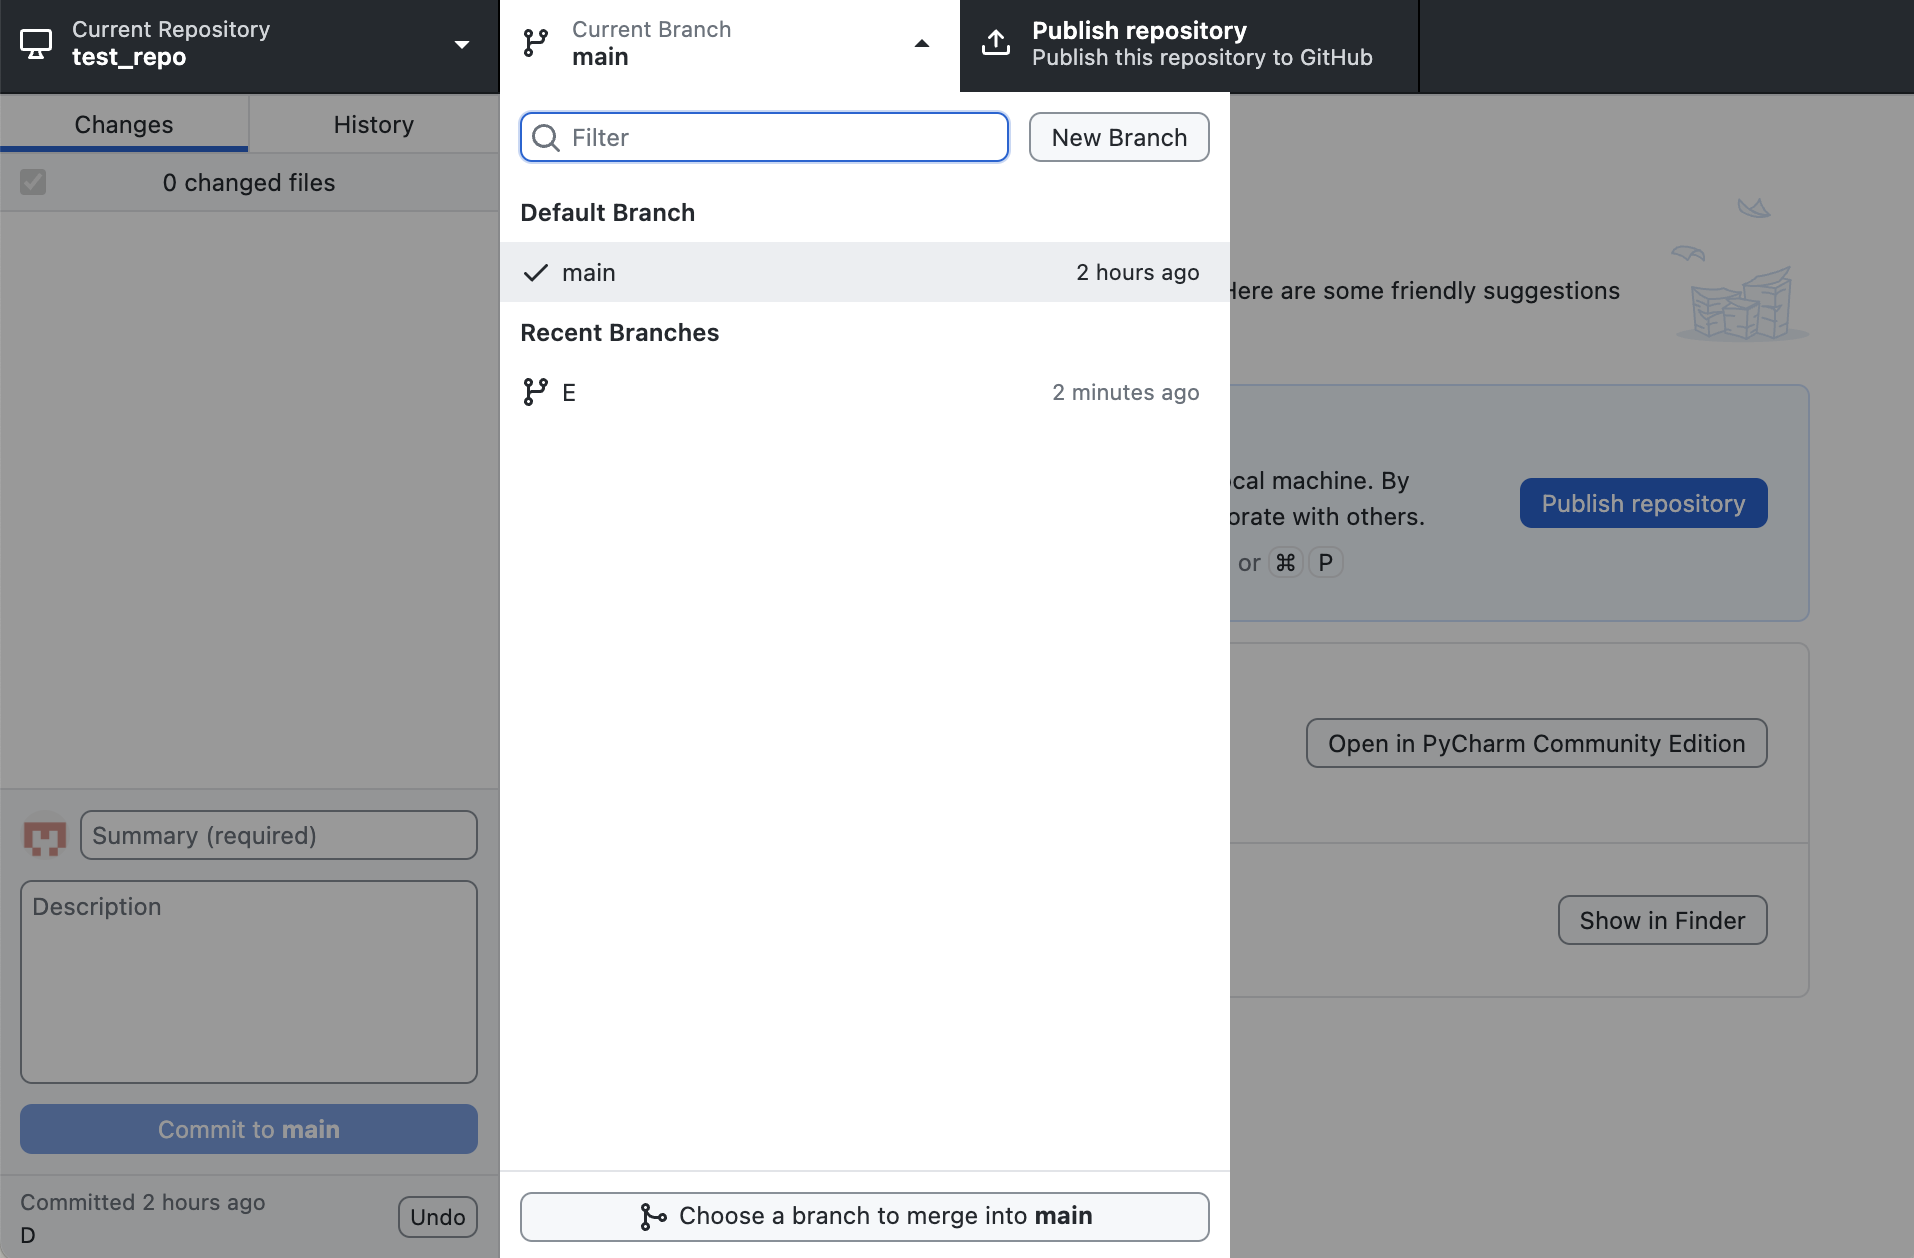
\includegraphics[width=\linewidth]{11.png}
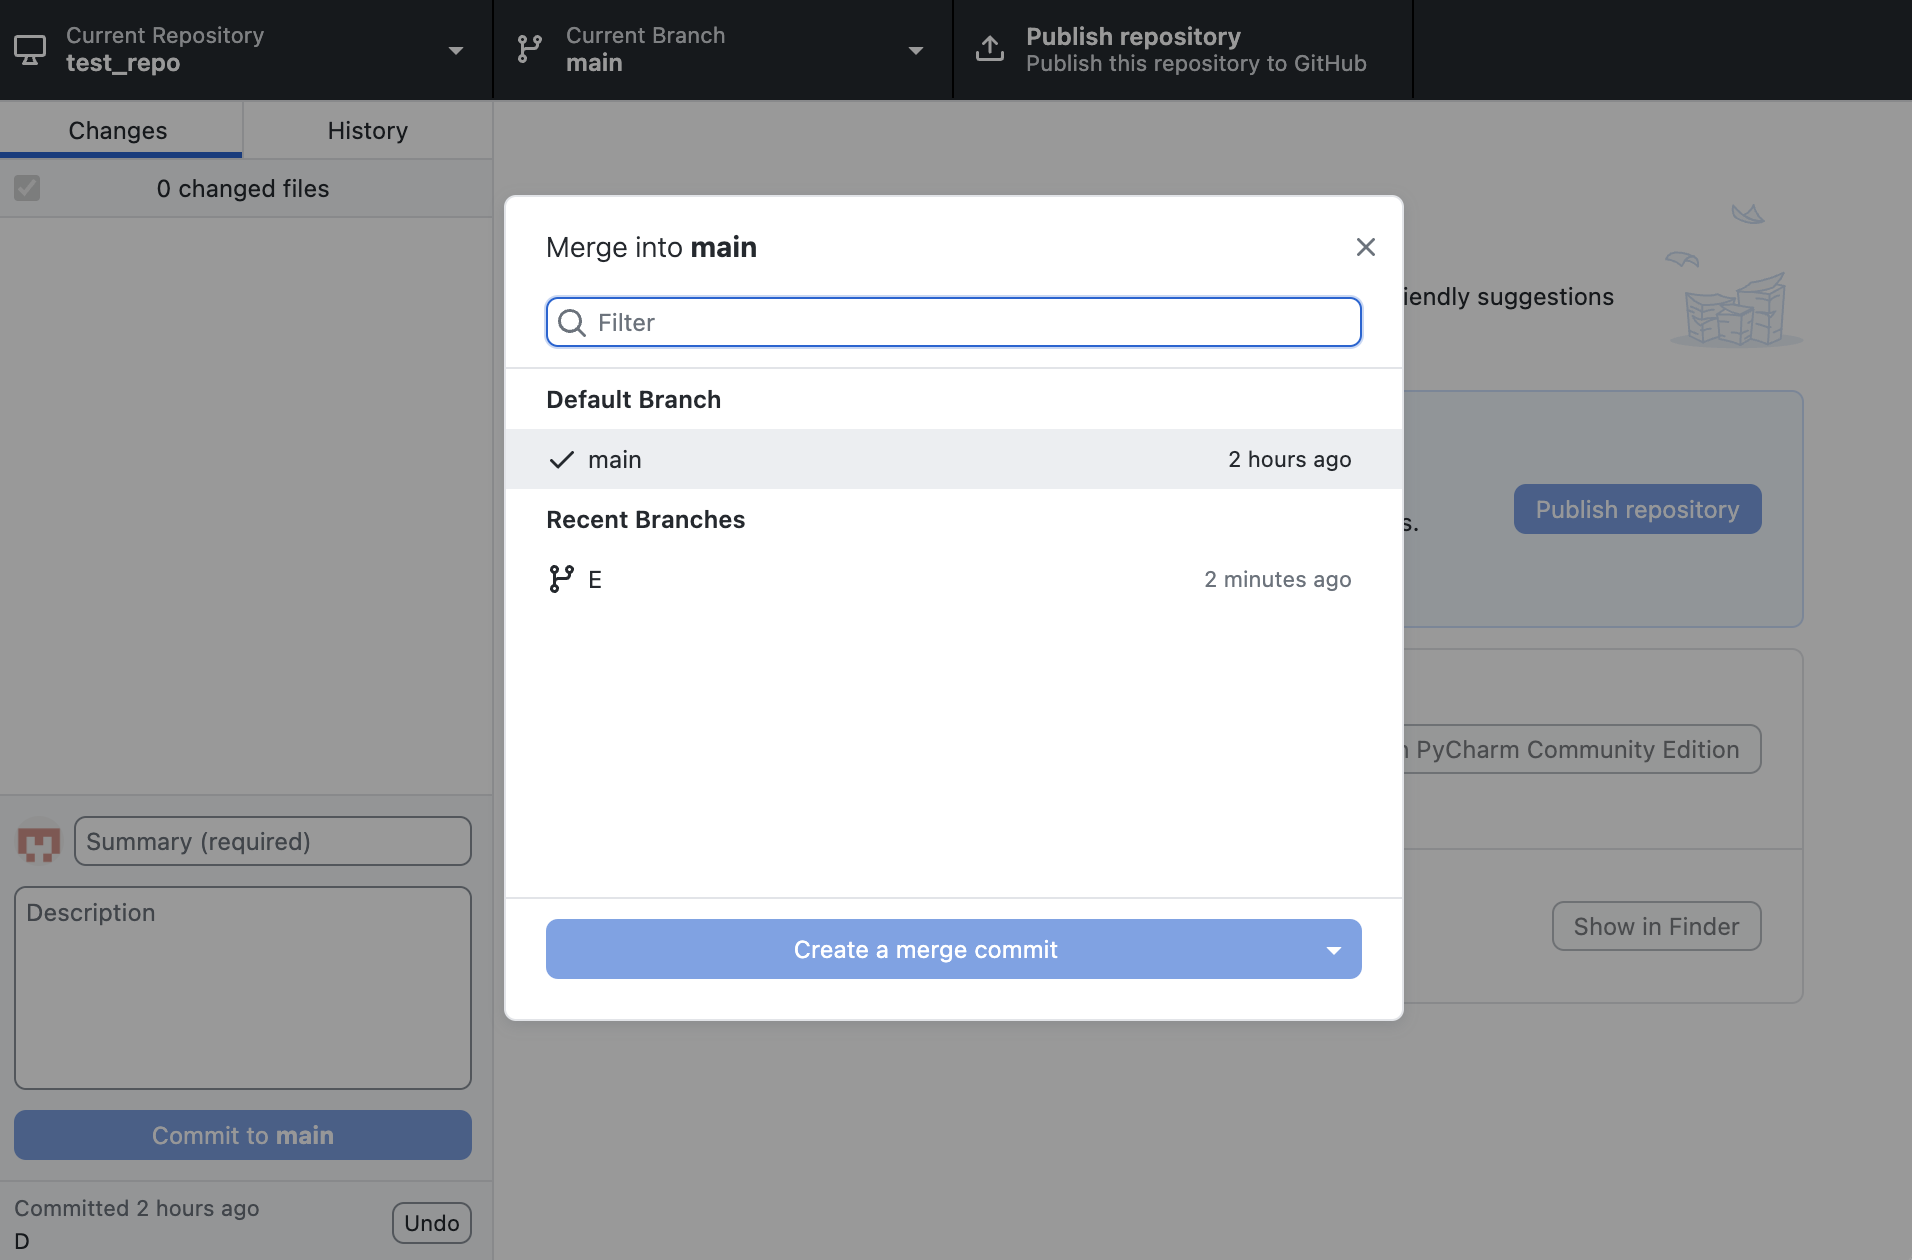
\includegraphics[width=\linewidth]{12.png}



\item What is a merge conflict? When do they occur?

\medskip
Merge conflict occurs when changes cannot be automatically combined by git and must be manually resolved, this usually happens when two developers work on the same file and some of the changes they made overlap. For example two developers working on different branches making different changes to the same line of code.
\medskip

\item Starting with an empty repository, despite a sequence of commands/actions that would result in a merge conflict. Include the exact edits and \texttt{git} commands or screenshots of the graphical git interface. Include the output or screenshot that shows the resulting merge conflict.

\medskip
Following question 2.2 4 to create a branch, from there make some changes to the branch and make a commit, then switch to the main branch and make some different changes to the same file you made changes to in the branch, then attempt to merge and you will be met with an error.

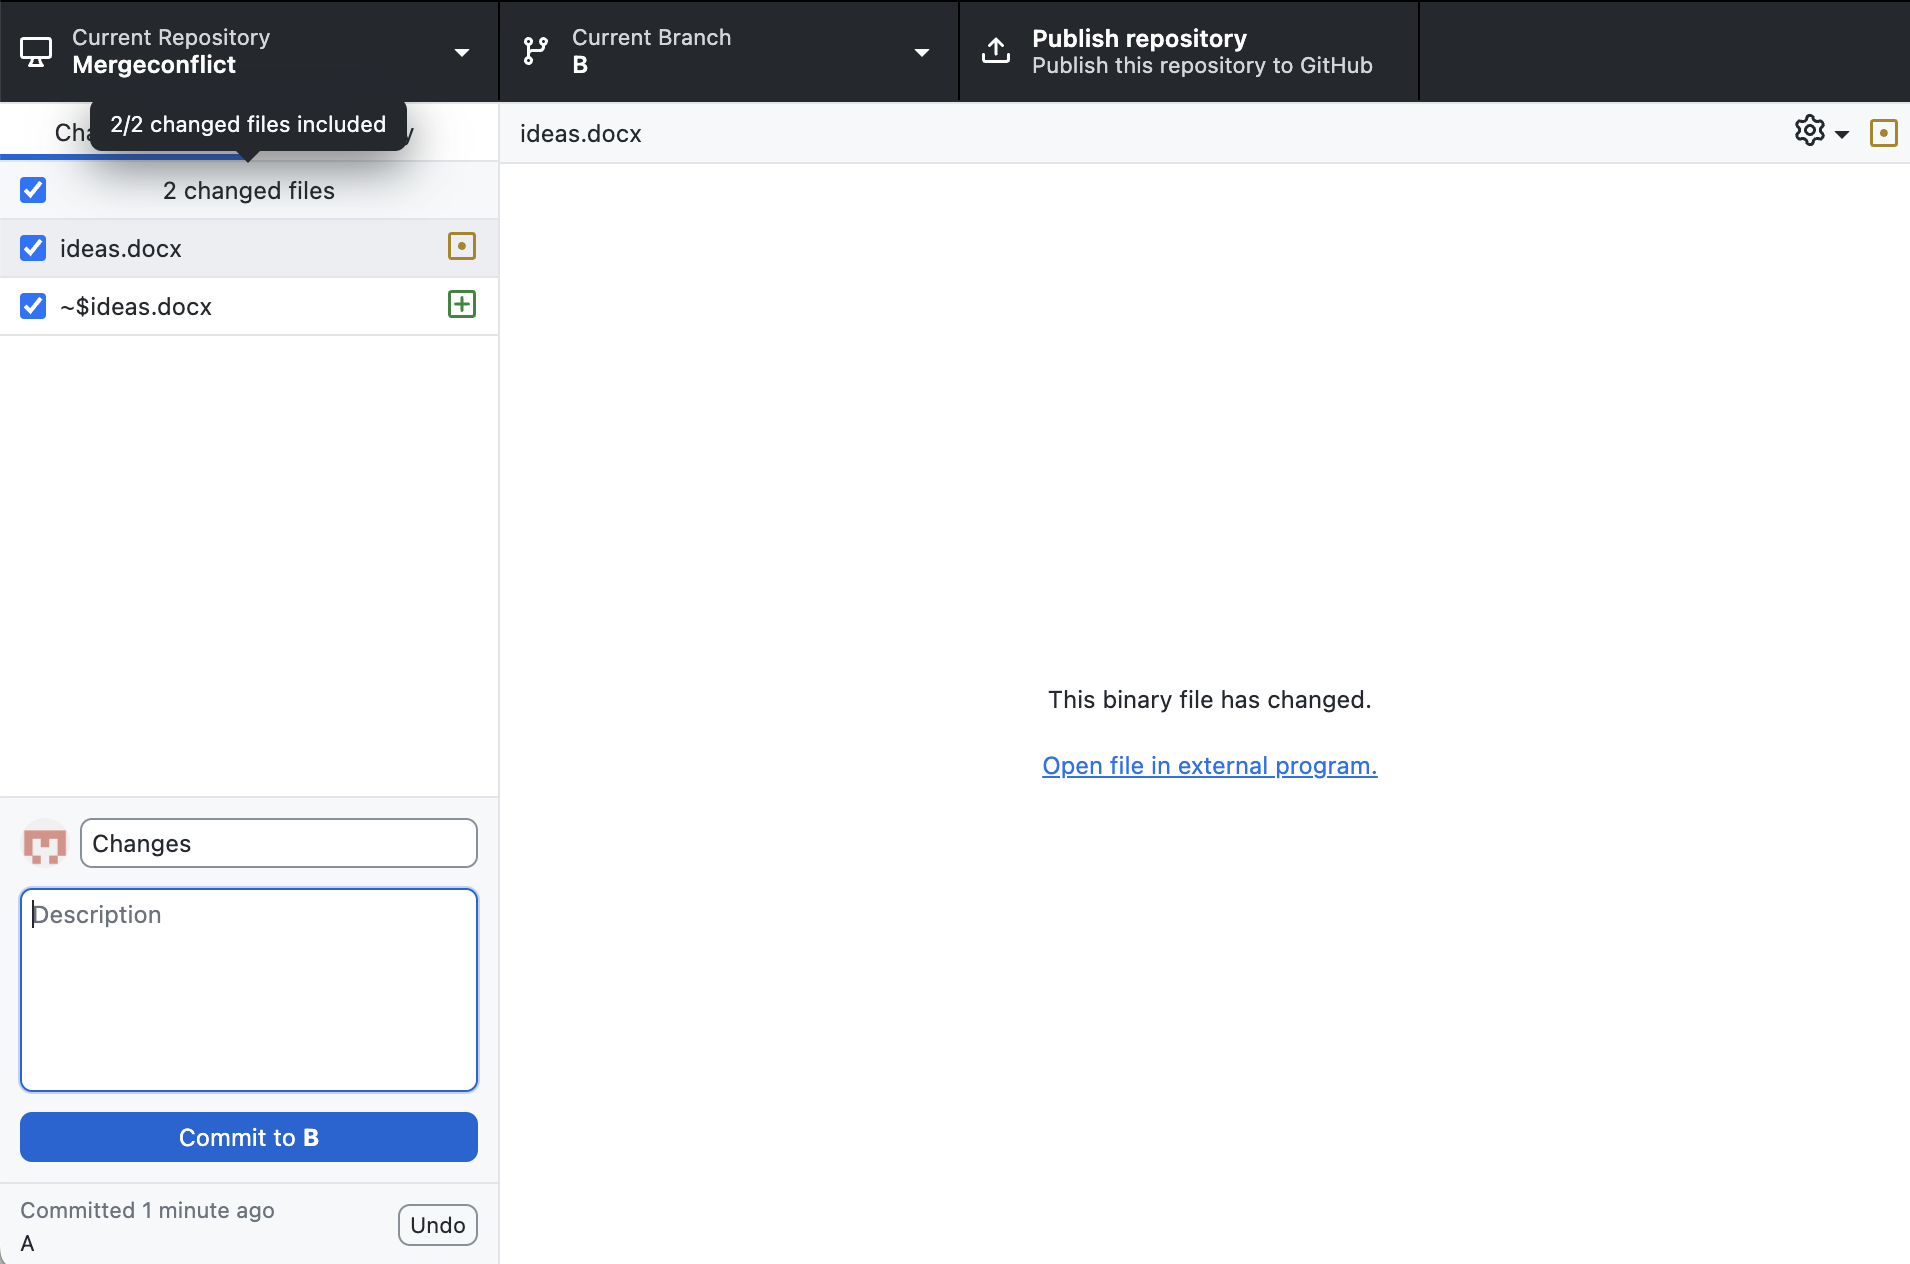
\includegraphics[width=\linewidth]{13.png}
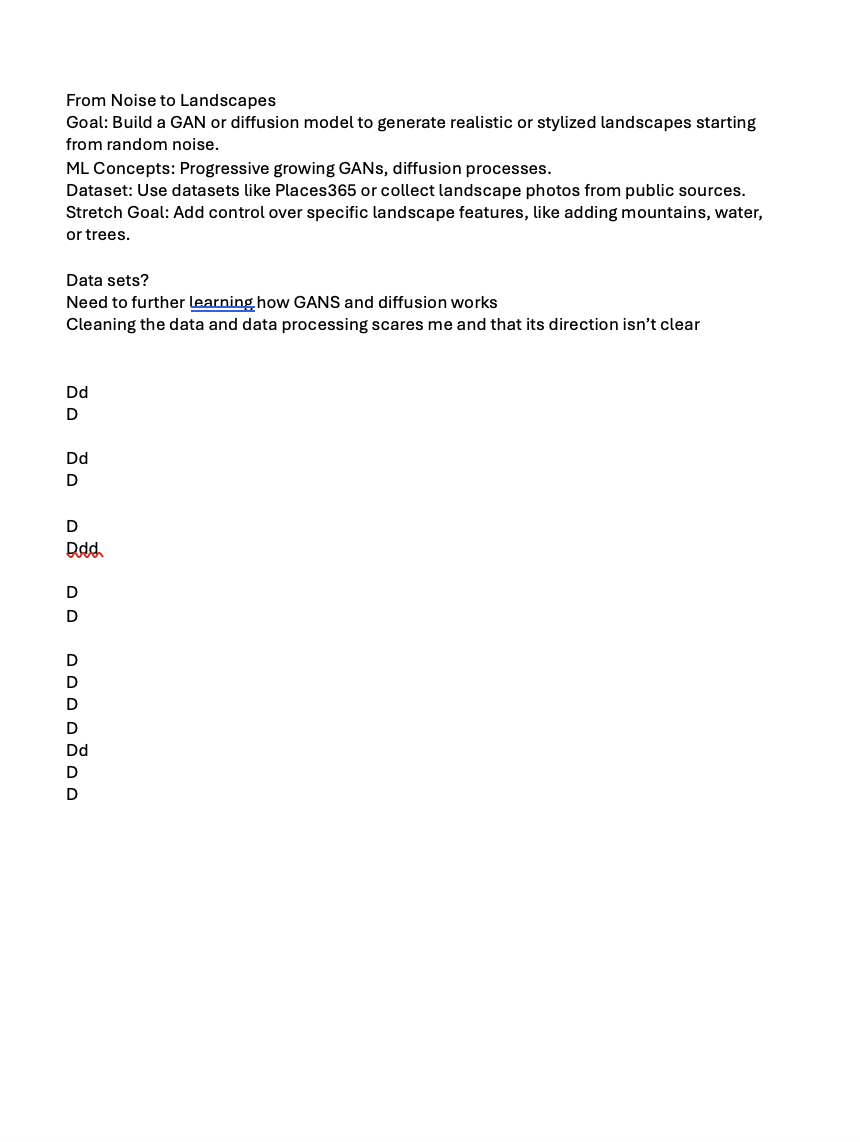
\includegraphics[width=\linewidth]{14.png}
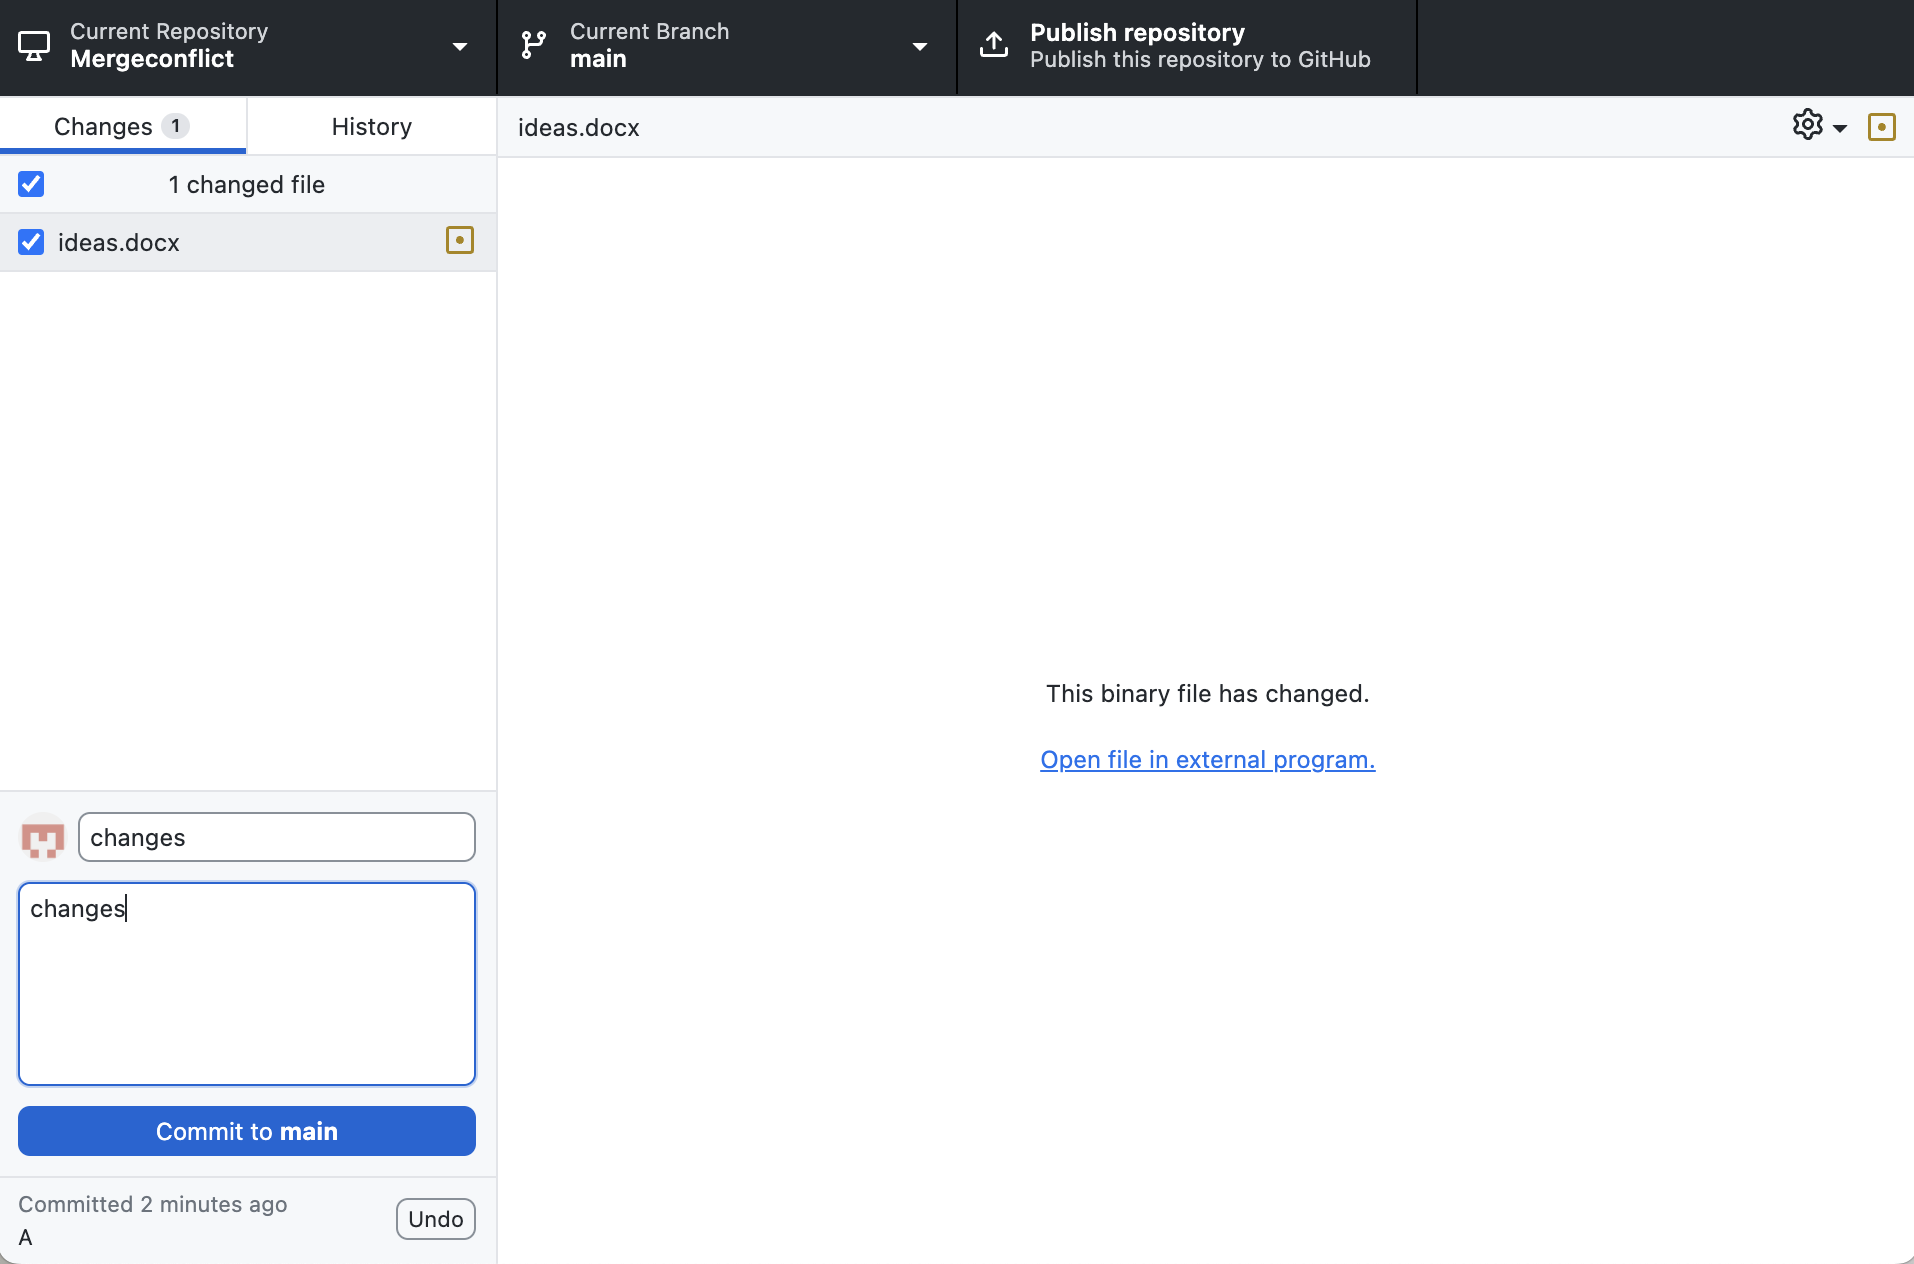
\includegraphics[width=\linewidth]{15.png}
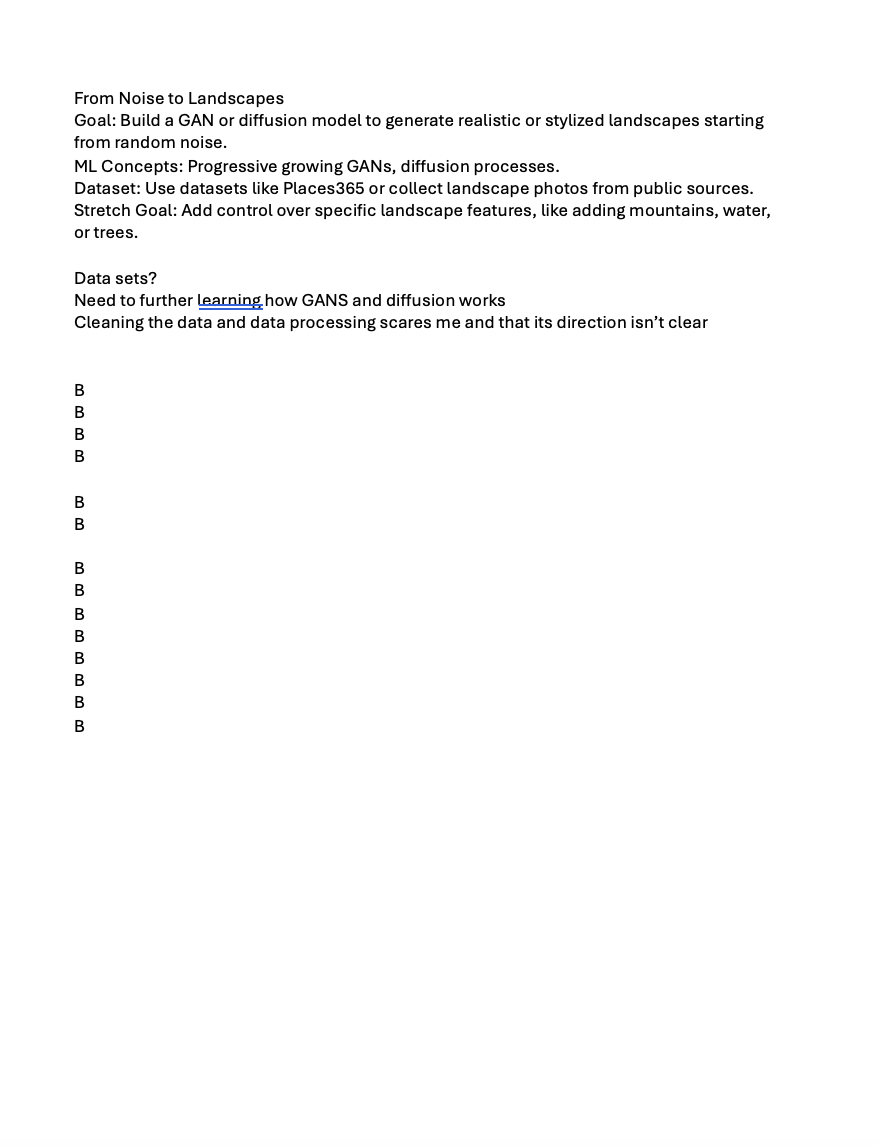
\includegraphics[width=\linewidth]{16.png}
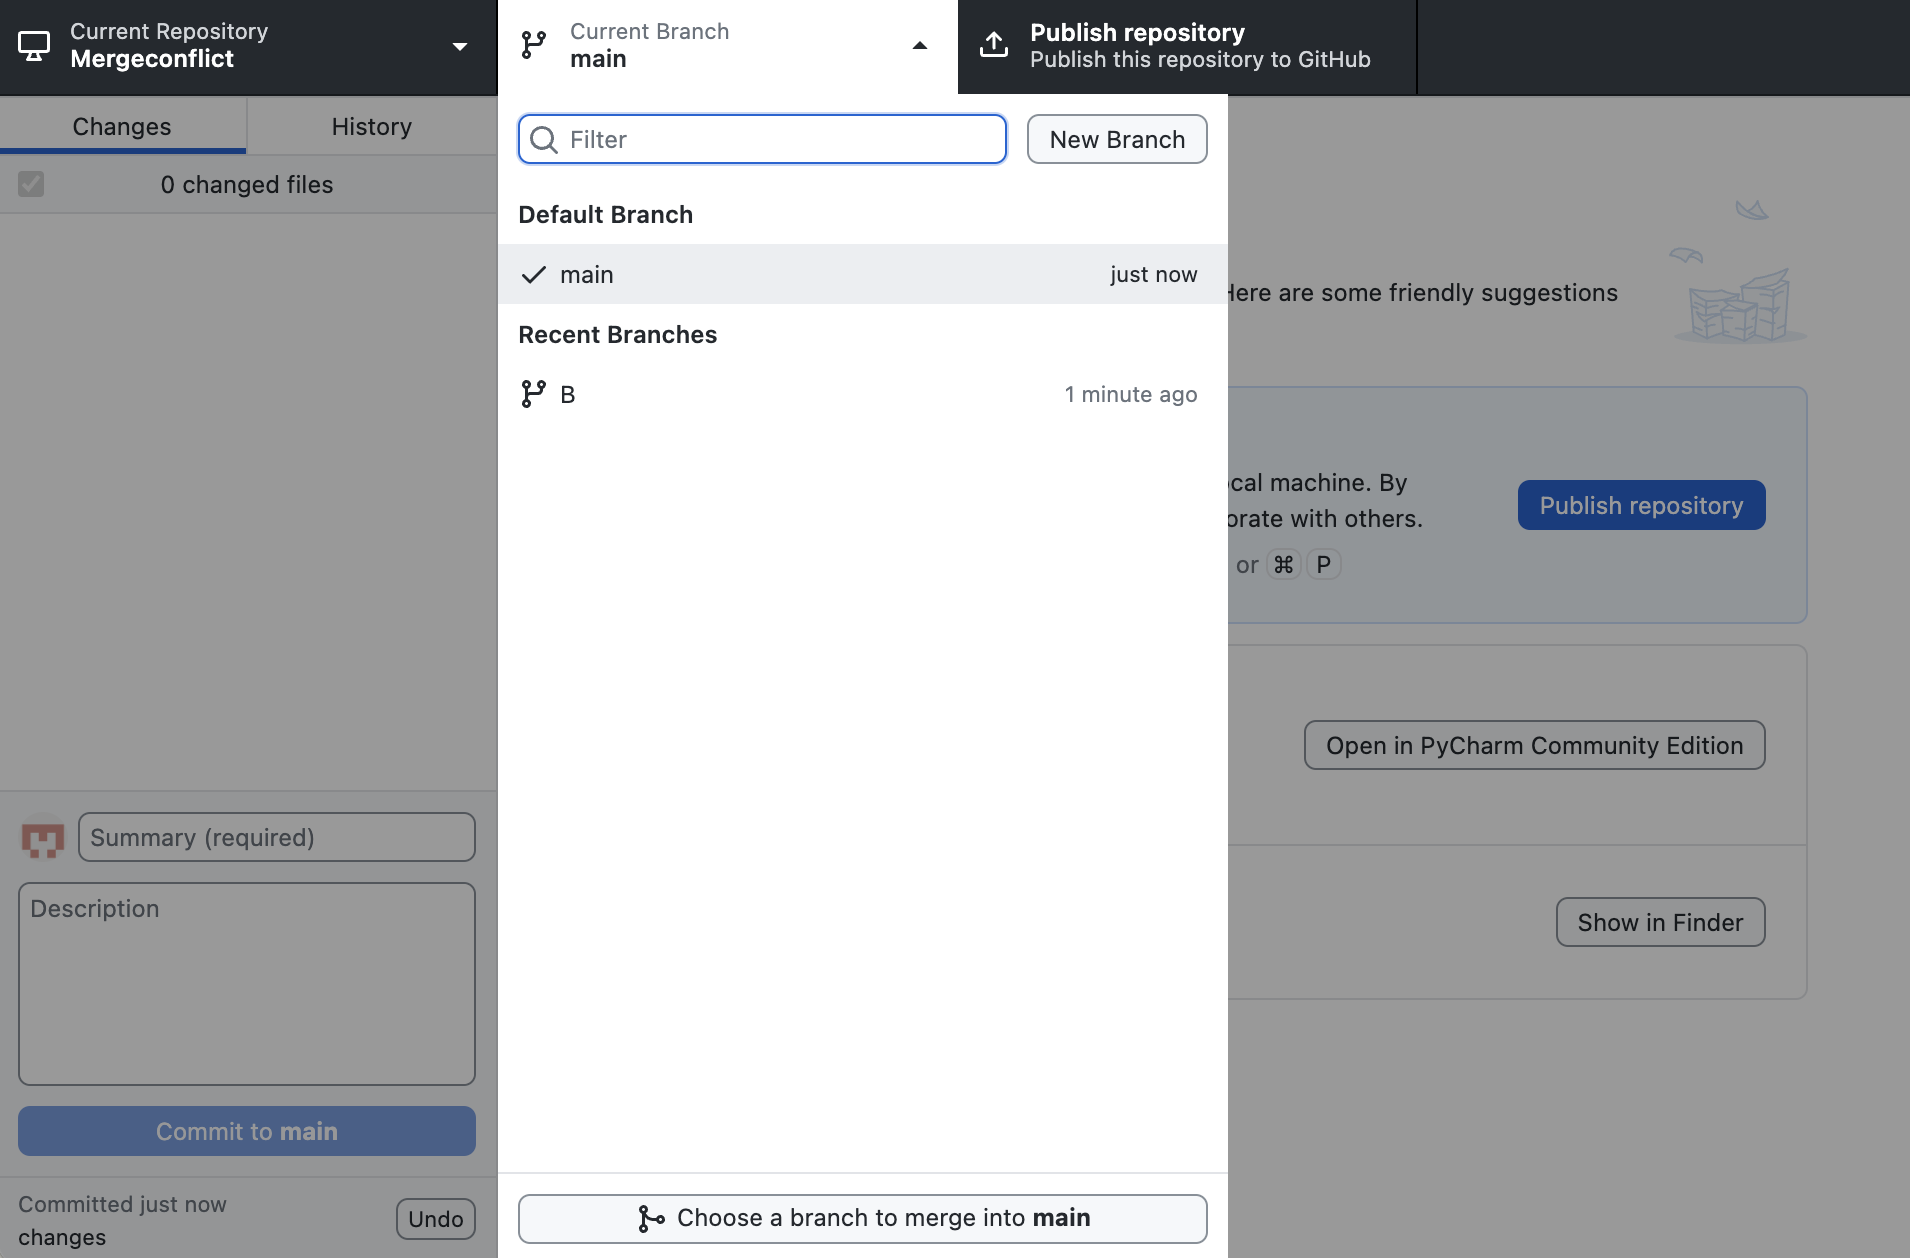
\includegraphics[width=\linewidth]{17.png}
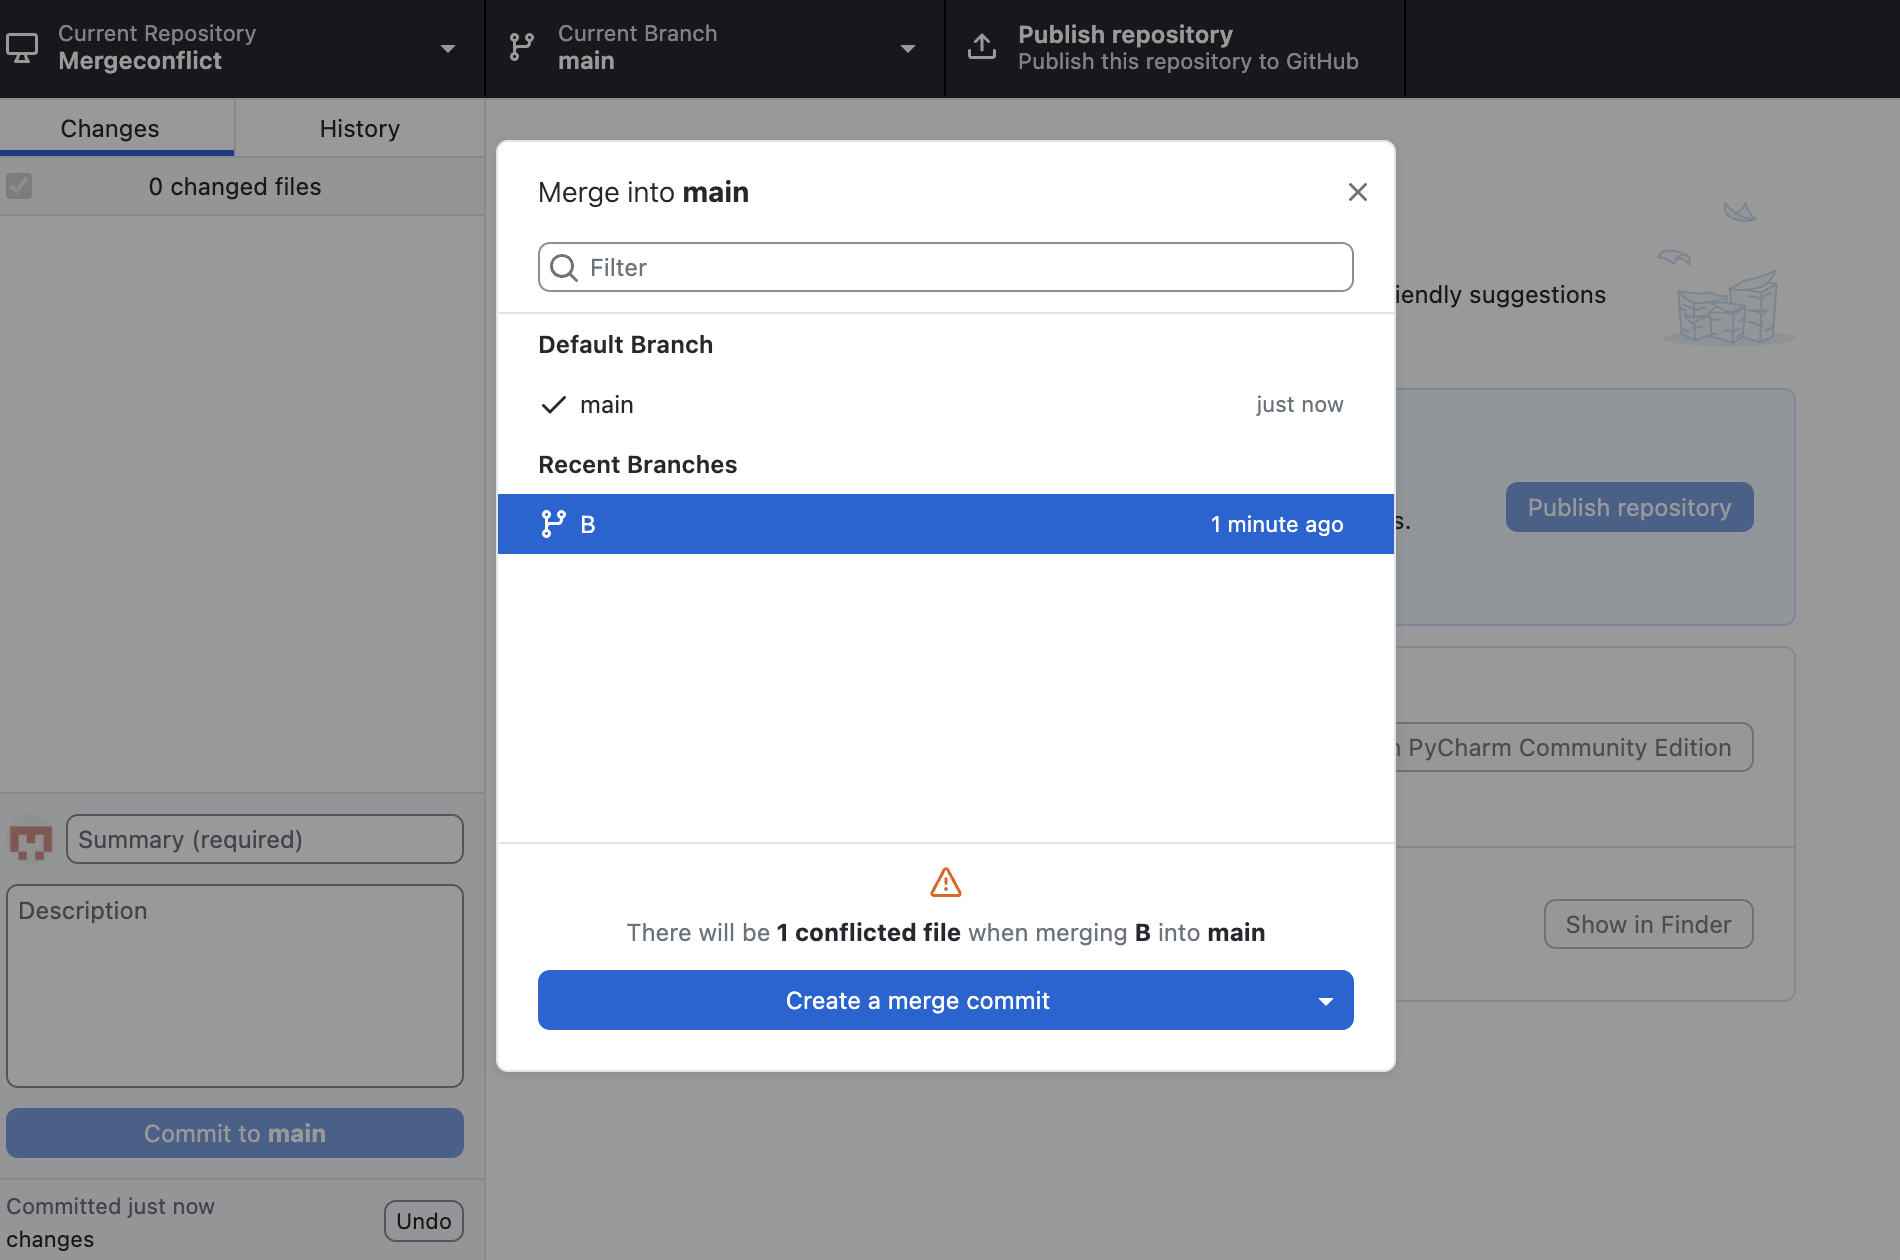
\includegraphics[width=\linewidth]{18.png}

\medskip

\end{enumerate}

\subsection{Remotes}

\begin{enumerate}
\item What is a remote?

\medskip
A remote is a link to a repository that is not hosted on the local device, or hosted on a remote server such as github. It allows push and pulls between the local and online repository
\medskip

\item What does pushing and pulling do?

\medskip
push uploads local changes to the remote repository, it only sends the committed changes to from the local branch that is being worked on to the corresponding branch.

pull checks the remote repository for commits not on the local repository and adds them to your repository through merging.
\medskip

\item Imagine you created a git repository for your project on your laptop and commit regularly, but only push your code to GitHub once a week on Sundays. Your laptop caught on fire on Friday. What can you do to get your code back?

\medskip
you can only get back the code you uploaded to the remote repo so the only code you can get back is the one that was pushed on Sunday. To get this code back us the pull command to pull from the remote repo.
\medskip

\end{enumerate}

\section{\LaTeX}

Find a source of each of the following types and add it to \texttt{references.bib}, with the appropriate data. Your sources do not have to relate to your project. Looking at \textcite{OverleafBibliographyManagement} and \textcite{WikipediaBibtex} may be helpful,

\begin{itemize}
\item a journal article
\item a conference article
\item a PhD or Master's thesis
\item an article in an edited popular media venue (newspaper, magazine, etc.)
\item a book
\item a chapter of a book
\item a YouTube video
\item a piece of technical documentation (e.g., a programming language reference, and API documentation, etc.)
\end{itemize}

Additionally, in you own words, explain the difference between \texttt{{\textbackslash}cite\{\}} and \texttt{{\textbackslash}textcite\{\}}. When should they each be used? Demonstrate your answers by using one of them with each of your references from above.

\medskip
first command produces a parenthetical citation which usually includes an author and year. For example:

\cite{Darroch.2017}

The second command does the same thing but the authors name is not in parenthesis only the year, this is to integrate the reference as part of the sentence. For example:

\textcite{youtube} is a trailer for an upcoming video game.
\medskip

\printbibliography

\end{document}
